%==================================
% SMDS TEMPLATE 
%==================================
% This document is a simplified template for preparing manuscripts for the Statistical Modeling and Data Science (SMDS) journal. The template provides basic structural elements for article preparation, including metadata, author affiliations, equations, tables, figures, and references. Authors may adapt this template to suit the requirements of their manuscript.

\documentclass[11pt,twoside]{article}

%==================================
% PACKAGES
%==================================
\usepackage{titlesec}
\titlespacing*{\section}{0pt}{1.5ex plus 0.5ex minus 0.2ex}{0.8ex plus 0.2ex}
\titlespacing*{\subsection}{0pt}{1.2ex plus 0.5ex minus 0.2ex}{0.5ex plus 0.2ex}

\usepackage[utf8]{inputenc}
\usepackage{amsmath,amssymb}
\usepackage[T1]{fontenc}
\usepackage{lmodern}
\usepackage{graphicx}
\usepackage{geometry}
\geometry{margin=1in}
\usepackage{booktabs}
\usepackage{array}
\usepackage{tabularx}
\usepackage{longtable}
\usepackage{adjustbox}
\usepackage{float}
\usepackage{caption}
\usepackage{placeins}
\usepackage{subcaption}
\usepackage{csquotes}
\usepackage[
backend=biber,
style=numeric-comp,
sorting=none,
giveninits=true,
doi=true,
url=true
]{biblatex}
\addbibresource{SMDSBib.bib}
\usepackage{fancyhdr}
\newcommand{\shorttitle}{}
\newcommand{\shortauthor}{}
\pagestyle{fancy}
\fancyhf{}
\fancyhead[L]{\small\shorttitle}
\fancyhead[R]{\small\shortauthor}
\fancyfoot[C]{\thepage}

\usepackage[colorlinks=true,allcolors=blue]{hyperref}
\newcommand{\orcidlink}[1]{%
\href{https://orcid.org/#1}{
\includegraphics[height=1.6ex]{ORCID_iD.png}}%
}

\graphicspath{{figures/}}
\captionsetup{font=small,labelfont=bf}
\setlength{\parindent}{1.2em}
\setlength{\parskip}{0.25em}
\sloppy

%==================================
% SIMPLE SMDS MACROS (Compatibility Layer)
%==================================

\newcommand{\SMDStitle}[1]{\title{\bfseries #1}}
\newcommand{\SMDSshorttitle}[1]{\def\shorttitle{#1}}
\newcommand{\SMDSshortafill}[1]{\def\shortauthor{#1}}

\newcommand{\SMDSaffilone}[1]{\def\affilone{#1}}
\newcommand{\SMDSaffiltwo}[1]{\def\affiltwo{#1}}
\newcommand{\SMDSaffilthree}[1]{\def\affilthree{#1}}
\newcommand{\SMDSaffilfour}[1]{\def\affilfour{#1}}
\newcommand{\SMDSaffilfive}[1]{\def\affilfive{#1}}

\newcommand{\SMDSauthorone}[4]{\def\authorone{#1$^{#2}$\,\orcidlink{#3}}}
\newcommand{\SMDSauthortwo}[4]{\def\authortwo{#1$^{#2}$\,\orcidlink{#3}}}
\newcommand{\SMDSauthorthree}[4]{\def\authorthree{#1$^{#2}$\,\orcidlink{#3}}}
\newcommand{\SMDSauthorfour}[4]{\def\authorfour{#1$^{#2}$\,\orcidlink{#3}}}
\newcommand{\SMDSauthorfive}[4]{\def\authorfive{#1$^{#2}$\,\orcidlink{#3}}}
\newcommand{\SMDSauthorsix}[4]{\def\authorsix{#1$^{#2}$\,\orcidlink{#3}}}

\newcommand{\SMDScorrespoding}[2]{%
\def\corrauthor{#1 \href{mailto:#2}{#2}}}

\newcommand{\SMDSKeywords}[1]{
\vspace{0.5em}
\noindent\textbf{Keywords:} #1
}

\newcommand{\acknowledg}[1]{
\section*{Acknowledgments}
#1
}

\newcommand{\funding}[1]{
\section*{Funding}
#1
}


%==================================
% METADATA
%==================================

\SMDStitle{Sensitivity Analysis of Global Digital Elevation Models for Machine Learning-Based Flood Susceptibility Mapping Using Google Earth Engine: A Controlled Comparative Study of SRTM, Copernicus DEM GLO-30, and ALOS AW3D30 in the Semarang--Demak Coastal Area}

\SMDSshortafill{M. I. A. Hakim and A. G. Z. Fann}
\SMDSshorttitle{Global DEM Sensitivity in Flood Susceptibility Mapping}

\SMDSaffilone{Department of Statistics and Data Science, Faculty of Mathematics and Natural Sciences, Universitas Negeri Semarang, Indonesia}


%----------------------------------
% AUTHORS
%----------------------------------
% Each author must provide a valid ORCID iD (16-digit format).
% Register at: https://orcid.org/register
% Format: \SMDSauthorX{Name}{AffiliationID}{ORCID}{email}

\SMDSauthorone{M Irfan Al Hakim}{1}{0009-0005-1222-7960}
{mirfanhakim25@students.unnes.ac.id}

\SMDSauthortwo{Alverrell Gustivierda Zidna Fann}{1}{0009-0002-5764-3229}
{alverrell@students.unnes.ac.id}

\SMDScorrespoding{$^*$Corresponding author, email:}{%
    mirfanhakim25@students.unnes.ac.id;
}

%==================================
% AUTHOR BLOCK
%==================================

\author{
\begin{minipage}{\textwidth}
\authorone,
\authortwo
\\[1em]
$^1$ \affilone\\
\corrauthor
\end{minipage}
}

%==================================

\date{\vspace{-1.5em}}
\begin{document}

\maketitle

%==================================
\begin{abstract}
Global Digital Elevation Models (DEMs) at 30-meter resolution are widely used as topographic inputs for data-driven flood susceptibility mapping where high-resolution LiDAR data are unavailable. However, global DEM products originate from distinct sensor missions and vertical datums, introducing surface representation differences that propagate into machine learning predictions. This study quantifies the sensitivity of Random Forest flood susceptibility mapping to the choice of global elevation product---Shuttle Radar Topography Mission (SRTM), Copernicus DEM GLO-30, and ALOS World 3D 30m (AW3D30)---in the low-lying Semarang--Demak coastal plain, Indonesia. Using a strict single-factor controlled experimental design in Google Earth Engine and Python, we lock the Sentinel-1 SAR proxy flood inventory (March 2024 event), 19 non-DEM environmental and land-cover predictors, a balanced master sample ($n = 5{,}956$; 2,978 flood and 2,978 non-flood points), train--test partitions, and Random Forest hyperparameters across all three treatments, varying only the five DEM-derived topographic predictors (elevation, slope, circular aspect sine and cosine, and aspect validity). Empirical results demonstrate that all three DEM configurations achieve strong discrimination under both stratified random holdout evaluation ($\text{ROC-AUC} = 0.932\text{--}0.940$) and four-fold spatial block cross-validation across 16 coordinate-quantile blocks ($\text{ROC-AUC} = 0.870\text{--}0.890$). Paired 16-block spatial bootstrap resampling (1,000 iterations) confirms a modest but statistically consistent advantage for Copernicus DEM GLO-30 over SRTM ($\Delta\text{AUC}_{\text{SRTM}-\text{GLO-30}} = -0.0155$, 95\% CI $[-0.0250, -0.0072]$) and ALOS AW3D30 ($\Delta\text{AUC}_{\text{GLO-30}-\text{AW3D30}} = +0.0108$, 95\% CI $[+0.0041, +0.0198]$), whereas SRTM and ALOS AW3D30 remain statistically indistinguishable ($\Delta\text{AUC} = -0.0047$, 95\% CI $[-0.0096, +0.0013]$). End-to-end replication across five independent random seeds confirms ranking stability ($\text{Spatial-CV AUC} = 0.889 \pm 0.013$ for GLO-30 vs.\ $0.877 \pm 0.017$ for AW3D30 and $0.869 \pm 0.017$ for SRTM). Despite small aggregate metric differences, AOI-masked raster comparisons ($1.44 \times 10^6$ valid pixels) reveal five-class agreement of 79.4\%--84.3\%, Very High risk ($p > 0.80$) area shifts from $100.58\text{ km}^2$ (SRTM) to $95.93\text{ km}^2$ (AW3D30, $-4.6\%$) and $109.63\text{ km}^2$ (GLO-30, $+9.0\%$) concentrated in shrubland (57.6\%--75.4\%), mangroves (62.6\%--74.9\%), and cropland (69.3\%--75.5\%), and significant Global Moran's $I$ in out-of-fold residuals ($0.355\text{--}0.377$, $p = 0.0001$).
\end{abstract}

\SMDSKeywords{flood susceptibility mapping, Digital Elevation Model sensitivity, SRTM, Copernicus DEM GLO-30, ALOS AW3D30, Random Forest, spatial block cross-validation, Semarang--Demak}

%==================================
\section{Introduction}\label{sec:introduction}

Flood susceptibility mapping estimates the spatial propensity of landscapes to experience inundation based on local topographic, hydrological, meteorological, and land-surface conditioning factors. Because relationships between flood occurrence and environmental controls are typically nonlinear and interactive, ensemble machine learning algorithms---particularly Random Forest \cite{breiman2001}---have become a standard methodological choice for regional susceptibility modelling \cite{saha2021,avand2022,hakim2026}. In low-lying coastal regions of developing countries, where high-resolution Airborne Laser Scanning (LiDAR) terrain models and field-surveyed flood boundaries are rarely available at regional scale, susceptibility workflows rely heavily on open-access satellite products hosted on cloud platforms such as Google Earth Engine (GEE) \cite{gorelick2017}.

A foundational dependency in these open-data workflows is the choice of global Digital Elevation Model (DEM). At the 30-meter spatial resolution commonly adopted in regional flood studies, three open global products are widely accessible: the Shuttle Radar Topography Mission (SRTM) derived from C-band Synthetic Aperture Radar (SAR) interferometry \cite{farr2007}, the Copernicus DEM GLO-30 derived from bistatic X-band TanDEM-X interferometry \cite{esa_glo30}, and the ALOS World 3D 30m (AW3D30) generated via optical stereo photogrammetry from the PRISM sensor \cite{tadono2016}. Although all three products share a nominal 30-meter grid spacing, they differ substantially in acquisition era, sensing physics, canopy and building penetration, void-filling procedures, and native vertical geoid datums (EGM96 for SRTM and ALOS AW3D30 versus EGM2008 for Copernicus GLO-30). In a comprehensive global benchmark against 65 LiDAR reference surveys across flood-prone environments, Meadows et al.\ \cite{meadows2024} demonstrated that vertical errors across SRTM, Copernicus DEM, AW3D30, NASADEM, and FABDEM vary systematically with terrain slope and land-cover class, concluding that no single global DEM is universally optimal across all flood landscapes.

Several recent studies have investigated how DEM selection or spatial resolution affects flood modelling outputs. In hydraulic and deep-learning inundation studies, DEM resolution and source differences have been shown to alter simulated flood extents, depths, and risk estimates \cite{ali2015,fatdillah2022,fereshtehpour2024,adesina2025,fikri2026,salgado2026}. Within data-driven flood susceptibility mapping, Avand et al.\ \cite{avand2022} and Saha et al.\ \cite{saha2021} examined spatial resolution effects on machine learning performance, while Tique et al.\ \cite{Tique2026} recently compared four DEM products, multiple hydrological delineation methods, and three machine learning classifiers for open-data flood susceptibility mapping in Nigeria. However, when experimental designs simultaneously vary the DEM source, the hydrological extraction method, and the machine learning algorithm, the specific contribution of the elevation source cannot be cleanly isolated from algorithmic or preprocessing variance.

In our previous baseline study published in \emph{Statistical Modeling and Data Science} \cite{hakim2026}, we developed a reproducible cloud-based workflow for the Semarang--Demak coastal plain in Central Java, Indonesia, combining a Sentinel-1 SAR change-detection flood inventory with multi-source GEE predictors across seven tree-based ensemble learners. That baseline investigation established that Random Forest achieved the highest point discrimination ($\text{ROC-AUC} = 0.852$) and was statistically indistinguishable from the other top ensemble learners under DeLong and bootstrap tests. Building directly upon that baseline, the present study shifts the analytical focus from \emph{algorithmic comparison} to \emph{controlled DEM-source sensitivity}. Rather than re-evaluating multiple classifiers, we lock Random Forest as the controlled modelling algorithm and hold the study boundary, Sentinel-1 flood inventory, non-DEM predictors, sampling design, and hyperparameter configuration strictly constant, isolating the global elevation product (SRTM, Copernicus DEM GLO-30, and ALOS AW3D30) as the sole experimental treatment.

The Semarang--Demak coastal area provides a rigorous testbed for DEM sensitivity analysis because its flood regime operates across a gentle coastal-alluvial gradient coupled with agricultural polders, aquaculture ponds, dense urban settlements, river corridors, and severe land subsidence \cite{marfai2008,abidin2015,Husnayaen2018,yuwono2024,verdyansyah2025,Sakina2025}. In such low-relief coastal zones, metric-scale vertical offsets or subtle slope differences among global DSM-like elevation products can materially shift predicted susceptibility classes. Furthermore, because spatially proximate sample pixels share autocorrelated environmental features, standard random train--test splits can inflate performance estimates and mask or exaggerate treatment differences \cite{roberts2017,ploton2020}. We therefore pair standard holdout evaluation with four-fold spatial block cross-validation, paired block bootstrap inference, and five-seed end-to-end replication.

Specifically, this study addresses four research questions:
\begin{enumerate}
\item How do the intrinsic sensor and datum characteristics of SRTM, Copernicus DEM GLO-30, and ALOS AW3D30 manifest in derived topographic parameters (elevation, slope, and circular aspect) across the Semarang--Demak coastal plain?
\item How does replacing the elevation source for the five DEM-derived predictors affect Random Forest flood susceptibility predictions under a strictly controlled experimental design?
\item How sensitive are model discrimination metrics and wall-to-wall spatial susceptibility patterns to DEM substitution when accounting for spatial autocorrelation via block cross-validation, block bootstrap resampling, and multi-seed testing?
\item Does the spatial sensitivity of flood susceptibility maps to DEM selection vary systematically across ESA WorldCover land-cover classes?
\end{enumerate}

\begin{table}[!htbp]
\small
\centering
\caption{Positioning of the present controlled experiment relative to prior DEM and flood susceptibility studies.}
\label{tab:prior-studies}
\begin{adjustbox}{max width=\textwidth}
\begin{tabular}{>{\raggedright}p{3.0cm} >{\raggedright}p{3.6cm} >{\raggedright}p{3.8cm} >{\raggedright\arraybackslash}p{4.4cm}}
\toprule
\textbf{Study} & \textbf{Primary Focus} & \textbf{Adopted Concept} & \textbf{Advancement in Present Study} \\
\midrule
Fatdillah et al.\ (2022) \cite{fatdillah2022}; Fikri et al.\ (2026) \cite{fikri2026} & DEM resolution and source impacts on hydraulic flood modelling & Topographic input differences propagate into flood risk outputs & Evaluated within a controlled machine learning susceptibility framework \\
Meadows et al.\ (2024) \cite{meadows2024} & Global vertical accuracy of 30\,m DEMs against 65 LiDAR surveys & SRTM, Copernicus GLO-30, and AW3D30 errors vary with land cover and slope & Traces DEM differences through to wall-to-wall susceptibility maps and WorldCover strata \\
Yuwono et al.\ (2024) \cite{yuwono2024}; Verdyansyah et al.\ (2025) \cite{verdyansyah2025} & Flood hazard and ML susceptibility in Semarang and Demak & Regional coastal flood context and local conditioning factors & Systematically varies global DEM sources under identical model controls \\
Hakim et al.\ (2026) \cite{hakim2026} & Sentinel-1 SAR inventory + 7 ensemble models in Semarang--Demak & Sentinel-1 change-detection label protocol and Random Forest baseline & Locks Random Forest and isolates DEM source sensitivity with corrected AOI-wide non-flood sampling \\
Tique et al.\ (2026) \cite{Tique2026} & Multi-DEM, multi-hydrology, and multi-ML comparison in Nigeria & Empirical evidence that DEM selection alters susceptibility mapping & Controls classifier, inventory, and non-DEM predictors to isolate single-factor DEM effects \\
\bottomrule
\end{tabular}
\end{adjustbox}
\end{table}

%==================================
\section{Study Area and Data}\label{sec:study-area-data}

\subsection{Study Area}\label{subsec:study-area}

The Area of Interest (AOI) encompasses the administrative territories of Semarang City (\emph{Kota Semarang}) and Demak Regency (\emph{Kabupaten Demak}) on the northern coast of Central Java, Indonesia, defined via the FAO Global Administrative Unit Layers (GAUL) Level 2 dataset ($110.27^\circ\text{E}\text{--}110.83^\circ\text{E}$, $7.14^\circ\text{S}\text{--}6.71^\circ\text{S}$). At the 30-meter analysis grid in UTM Zone 49S (\texttt{EPSG:32749}), the AOI comprises $1{,}469{,}555$ pre-mask grid pixels and, after strict AOI polygon masking (\texttt{FAO/GAUL/2015/level2} Demak and Semarang City, geodesic area $1{,}310.09\text{ km}^2$), $1{,}444{,}085$ valid raster pixels ($1{,}299.84\text{ km}^2$ spherical / $1{,}299.68\text{ km}^2$ planar) for SRTM and Copernicus GLO-30 and $1{,}429{,}582$ valid pixels ($1{,}286.79\text{ km}^2$ spherical / $1{,}286.62\text{ km}^2$ planar) for ALOS AW3D30. Topographically, the region exhibits a sharp dichotomy between a broad, extremely flat northern coastal-alluvial plain (where elevations frequently lie below $5\text{ m}$ and slopes are below $2^\circ$) and steeper volcanic foothills in the southern portion of Semarang City rising above $230\text{ m}$. Because this coastal corridor experiences recurrent monsoon riverine overflows, drainage congestion, and coastal inundation \cite{marfai2008,abidin2015,Husnayaen2018}, minor vertical and slope discrepancies among global DEMs in the low-relief northern plain are particularly consequential for flood susceptibility delineation.

\subsection{Global Elevation Treatments and Multi-Source Geospatial Data}\label{subsec:data-sources}

All geospatial datasets were acquired and harmonized within Google Earth Engine \cite{gorelick2017} on a unified 30-meter grid in \texttt{EPSG:32749} (Table~\ref{tab:data-sources}). The three global elevation products serving as experimental treatments are:
\begin{enumerate}
\item \textbf{SRTM (\texttt{USGS/\allowbreak SRTMGL1\_003})} \cite{farr2007}: Acquired in February 2000 using single-pass C-band ($\lambda \approx 5.6\text{ cm}$) radar interferometry. Because C-band radar partially reflects from upper vegetation canopies and building roofs, SRTM behaves as a Digital Surface Model (DSM) referenced vertically to the EGM96 geoid.
\item \textbf{Copernicus DEM GLO-30 (\texttt{COPERNICUS/\allowbreak DEM/\allowbreak GLO30})} \cite{esa_glo30}: Derived from the TanDEM-X mission (2010--2015) using single-pass bistatic X-band ($\lambda \approx 3.1\text{ cm}$) radar interferometry, eliminating temporal decorrelation. It represents a high-consistency DSM referenced vertically to the EGM2008 geoid.
\item \textbf{ALOS AW3D30 v4.1 (\texttt{JAXA/\allowbreak ALOS/\allowbreak AW3D30/\allowbreak V4\_1})} \cite{tadono2016}: Reconstructed photogrammetrically from triplet panchromatic stereo imagery acquired by the PRISM optical sensor aboard ALOS (2006--2011) and referenced to the EGM96 geoid (matching SRTM, whereas Copernicus GLO-30 uses EGM2008). Because optical stereo matching can suffer from cloud-induced voids, we explicitly parsed the official mask band (\texttt{MSK}): across the Semarang--Demak AOI, the model retains only valid primary pixels ($\texttt{MSK}=0$), covering $1{,}429{,}582$ pixels ($1{,}286.79\text{ km}^2$ spheroidal; $99.0\%$ of the $1{,}444{,}085$-pixel AOI grid on SRTM/GLO-30), whereas cloud/void-filled pixels ($\texttt{MSK}=3$ and $48$) are not retained in the modeling. Retaining $\texttt{MSK}=0$ ensures that topographic derivatives reflect valid photogrammetric observations.
\end{enumerate}

\begin{table}[!htbp]
\small
\centering
\caption{Summary of multi-source satellite datasets, GEE asset identifiers, spatial resolutions, and analytical roles.}
\label{tab:data-sources}
\begin{adjustbox}{max width=\textwidth}
\begin{tabular}{>{\raggedright}p{2.7cm} >{\raggedright}p{2.8cm} >{\raggedright}p{1.6cm} >{\raggedright}p{4.3cm} >{\raggedright\arraybackslash}p{3.4cm}}
\toprule
\textbf{Dataset} & \textbf{Sensor / Nature} & \textbf{Native Grid} & \textbf{Provider \& GEE Asset ID} & \textbf{Analytical Role} \\
\midrule
Sentinel-1 GRD & C-band SAR (VH backscatter, dB) & 10\,m (IW) & ESA Copernicus; \texttt{COPERNICUS/\allowbreak S1\_GRD} & Locked binary flood inventory (March 2024 event) \\
SRTM GL1 v3 & C-band InSAR DSM (EGM96, m) & 30\,m & NASA/USGS; \texttt{USGS/\allowbreak SRTMGL1\_003} & Elevation Treatment 1 (5 topographic predictors) \\
Copernicus DEM GLO-30 & X-band bistatic InSAR DSM (EGM2008, m) & 30\,m & ESA Copernicus; \texttt{COPERNICUS/\allowbreak DEM/\allowbreak GLO30} & Elevation Treatment 2 (5 topographic predictors) \\
ALOS AW3D30 v4.1 & Optical stereo PRISM DSM (EGM96, m) & 30\,m & JAXA; \texttt{JAXA/\allowbreak ALOS/\allowbreak AW3D30/\allowbreak V4\_1} & Elevation Treatment 3 (5 topographic predictors) \\
MERIT Hydro v1.0.1 & Hydrologically conditioned hydrography & 90\,m & Univ.\ Tokyo \cite{yamazaki2019}; \texttt{MERIT/\allowbreak Hydro/\allowbreak v1\_0\_1} & Locked hydrological predictors (\texttt{hand}, \texttt{upa\_log}, \texttt{river\_width}, \texttt{dist\_river}) \\
JRC Global Surface Water & Long-term water occurrence (1984--2021, \%) & 30\,m & EC JRC \cite{pekel2016}; \texttt{JRC/\allowbreak GSW1\_4/\allowbreak Global\allowbreak SurfaceWater} & Permanent water mask ($\ge 80\%$) \& \texttt{dist\_perm\_water} \\
CHIRPS Daily & Infrared + station precipitation (mm) & $0.05^\circ$ ($\sim$5.5\,km) & UCSB CHG \cite{funk2015}; \texttt{UCSB-CHG/\allowbreak CHIRPS/\allowbreak DAILY} & Locked 7-day and 30-day antecedent rainfall \\
Sentinel-2 SR (L2A) & Multispectral optical reflectance & 10--20\,m & ESA Copernicus; \texttt{COPERNICUS/\allowbreak S2\_SR\_\allowbreak HARMONIZED} & Locked spectral indices (\texttt{ndvi}, \texttt{ndwi}, \texttt{mndwi}, \texttt{ndbi}) \\
ESA WorldCover v200 & Global land-cover classification (2021) & 10\,m & ESA \cite{zanaga2021}; \texttt{ESA/\allowbreak WorldCover/\allowbreak v200} & Locked land-cover dummy variables + spatial stratification \\
\bottomrule
\end{tabular}
\end{adjustbox}
\end{table}

%==================================
\section{Methodology}\label{sec:methodology}

\subsection{Single-Factor Controlled Experimental Design}\label{subsec:experimental-design}

To isolate the effect of the elevation source without confounding from classifier architecture or sample selection, we implemented a single-factor controlled experiment with three treatment levels: SRTM, Copernicus DEM GLO-30, and ALOS AW3D30 (Table~\ref{tab:experimental-design}). Across all three treatments, six core components are locked identically: (1) the binary Sentinel-1 flood inventory, (2) the AOI and 30-meter UTM Zone 49S analysis grid, (3) the 19 non-DEM predictors, (4) the master sample point coordinates and class balance ($n = 5{,}956$), (5) the train--test split and spatial cross-validation block assignments, and (6) the Random Forest hyperparameter settings.

\begin{table}[!htbp]
\small
\centering
\caption{Controlled experimental design isolating global DEM source sensitivity.}
\label{tab:experimental-design}
\begin{tabular}{>{\raggedright}p{4.5cm} >{\raggedright\arraybackslash}p{9.8cm}}
\toprule
\textbf{Experimental Component} & \textbf{Specification Across Treatments} \\
\midrule
Treatment factor & Global 30\,m elevation source: (1) SRTM, (2) Copernicus DEM GLO-30, (3) ALOS AW3D30 \\
Treatment-varying predictors (5) & $\text{elevation}_d$, $\text{slope}_d$, $\text{aspect\_sin}_d$, $\text{aspect\_cos}_d$, $\text{aspect\_valid}_d$ ($d \in \{\text{srtm}, \text{glo30}, \text{aw3d30}\}$) \\
Locked non-DEM predictors (19) & 11 continuous hydro-meteorological/spectral variables + 8 ESA WorldCover dummy variables \\
Locked supervisory label & Single Sentinel-1 VH change-detection flood inventory (March 2024 event) \\
Locked sampling & Stratified balanced master sample ($n = 5{,}956$: 2,978 flood, 2,978 non-flood; seed = 42) \\
Locked evaluation classifier & \texttt{scikit-learn} Random Forest (400 trees, \texttt{min\_samples\_leaf}=2, balanced class weights) \\
Locked spatial mapping classifier & GEE \texttt{smileRandomForest} (300 trees, \texttt{minLeafPopulation}=2, \texttt{bagFraction}=0.7; 17 raw inputs) \\
Validation \& sensitivity suite & 75:25 stratified holdout, 4-fold spatial block CV (16 blocks), 1,000-iteration block bootstrap, 5-seed replication, pixel-wise transitions, and WorldCover stratification \\
\bottomrule
\end{tabular}
\end{table}

\subsection{Sentinel-1 SAR Flood Inventory and Correction of Non-Flood Sampling Bias}\label{subsec:flood-inventory-sampling}

Following the validated protocol of our baseline study \cite{hakim2026} and UN-SPIDER guidelines \cite{islammeng2022,unspider2024}, the binary flood inventory was generated once from Sentinel-1 Interferometric Wide-swath (IW) Ground Range Detected (GRD) VH-polarized imagery covering the March 2024 Central Java flood event. Pre-event (25 February--12 March 2024) and post-event (15--31 March 2024) median composites were converted from decibels ($\text{dB}$) to linear power scale ($P = 10^{\text{dB}/10}$). A pixel was classified as flooded ($\text{flood}=1$) when five conditions were simultaneously satisfied: (i) pre-to-post VH power ratio $P_{\text{before}}/P_{\text{after}} > 1.25$; (ii) post-event backscatter $\text{VH}_{\text{after}} < -18\text{ dB}$; (iii) outside permanent water bodies defined by JRC Global Surface Water occurrence $\ge 80\%$ \cite{pekel2016}; (iv) terrain slope $< 5^\circ$ (computed from SRTM as a unified radar layover/foreshortening guard across all treatments); and (v) membership in a connected eight-direction cluster of at least 8 pixels at 30\,m resolution to suppress SAR speckle. Across the AOI, this procedure yielded $58{,}573$ flood-labelled pixels ($\approx 52.7\text{ km}^2$) and $1{,}410{,}981$ non-flood pixels (Figure~\ref{fig:study-area}a).

\begin{figure}[!htbp]
\centering
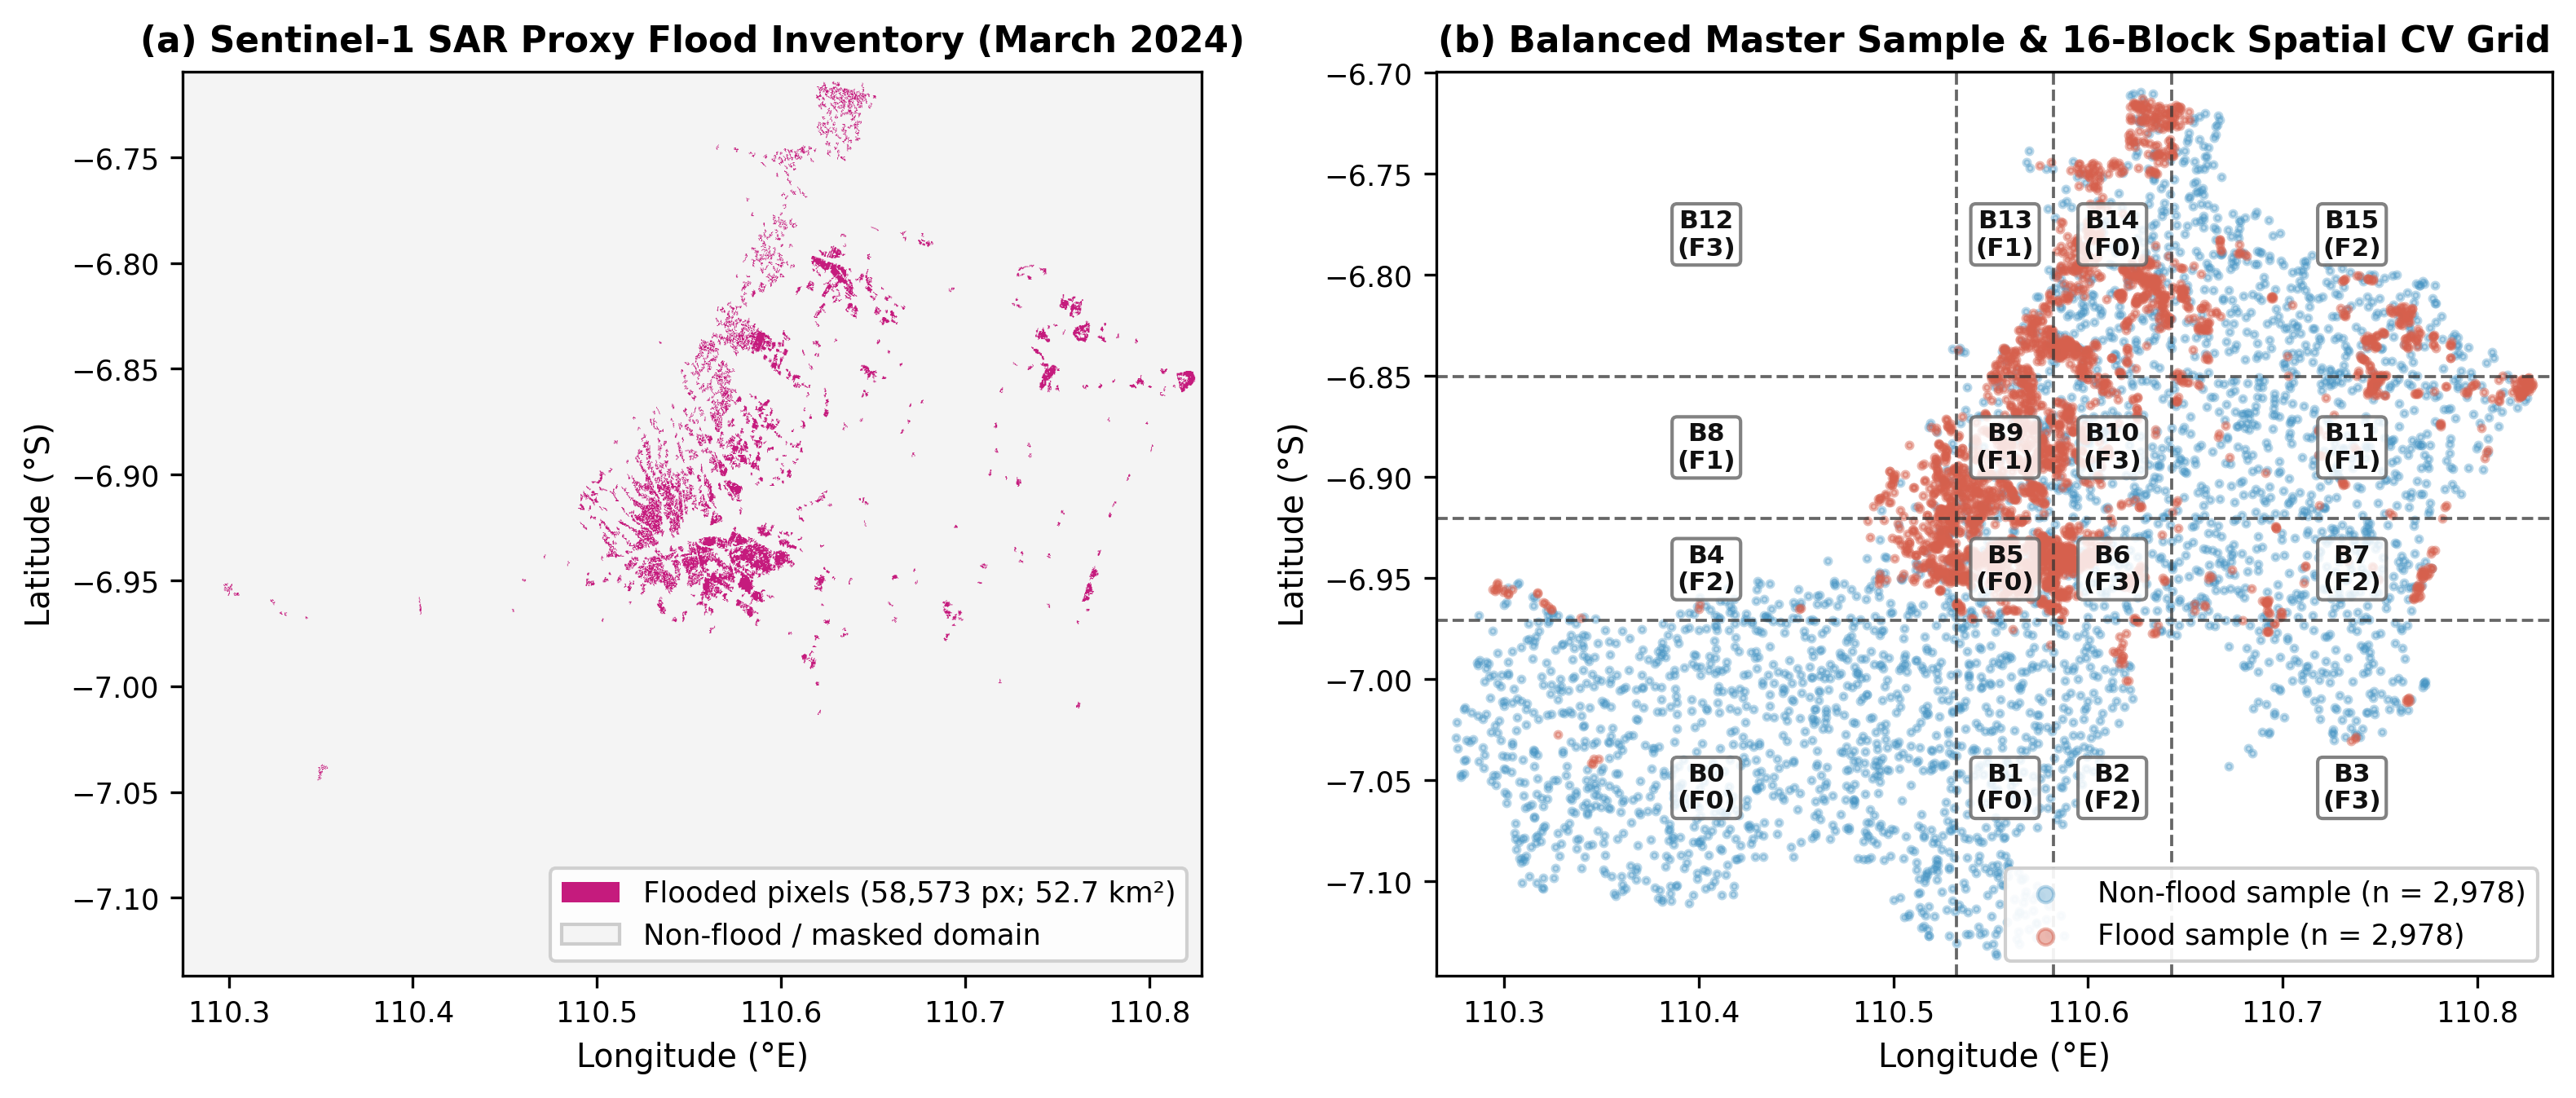
\includegraphics[width=0.94\textwidth]{figures/fig_study_area_samples.png}
\caption{Study area and sampling structure: (a) Sentinel-1 SAR proxy flood inventory for the March 2024 flood event in Semarang--Demak ($58{,}573$ flooded pixels); (b) spatial distribution of the balanced master sample ($n = 5{,}956$) partitioned into 16 coordinate-quantile blocks (\texttt{B0}--\texttt{B15}) and assigned to four spatial cross-validation folds (\texttt{F0}--\texttt{F3}).}
\label{fig:study-area}
\end{figure}

During diagnostic auditing of the sampling pipeline, we identified and corrected a critical geospatial masking pitfall associated with the JRC Global Surface Water \texttt{occurrence} band. In GEE, the JRC \texttt{occurrence} band is sparsely populated: valid non-null observations exist on only $187{,}777$ pixels ($12.78\%$ of the AOI), where water has been detected at least once since 1984. If permanent water masking is applied naively via \texttt{permanent\_water.Not()} without first unmasking no-data pixels, boolean negation preserves the null mask across upland and inland areas. Under such naive masking, the candidate pool for non-flood ($\text{flood}=0$) sampling collapses silently to $123{,}616$ pixels ($8.76\%$ of non-flood pixels) confined to a narrow coastal and riparian belt (mean sample elevation of $4.15\text{ m}$ versus the AOI mean of $42.7\text{ m}$). By explicitly applying \texttt{permanent\_water.unmask(0)} prior to negation---treating upland pixels without historical water detections as non-water---the valid non-flood candidate pool expands to $1{,}382{,}033$ pixels ($97.95\%$ of all non-flood pixels across the AOI). From this corrected domain, stratified random sampling extracted 3,000 candidate points per class; after multi-band extraction and complete-case filtering across all 27 raster bands, the balanced master sample comprises exactly $n = 5{,}956$ observations ($2{,}978$ flood and $2{,}978$ non-flood points; Figure~\ref{fig:study-area}b). It should be noted that Class 1 denotes pixels detected as flooded by the Sentinel-1 SAR proxy pipeline (which can only form within the $12.78\%$ JRC \texttt{occurrence} support footprint), whereas Class 0 (``non-flood'') denotes pixels not identified as flooded by the same proxy pipeline across $97.95\%$ of the non-flood AOI rather than ground-truth proof of non-inundation; model predictions outside JRC positive support therefore represent spatial extrapolation.

\subsection{Topographic Feature Engineering and Locked Non-DEM Predictors}\label{subsec:feature-engineering}

For each elevation treatment $d \in \{\text{srtm}, \text{glo30}, \text{aw3d30}\}$, five topographic features were computed on the common 30-meter \texttt{EPSG:32749} grid using \texttt{ee.Terrain}:
\begin{equation}
\mathbf{x}_{\text{DEM}}^{(d)} = \Bigl(\text{elevation}_d,\; \text{slope}_d,\; \sin(\alpha_d),\; \cos(\alpha_d),\; \mathbb{I}(\text{slope}_d > 0)\Bigr),
\label{eq:dem-features}
\end{equation}
where $\alpha_d \in [0^\circ, 360^\circ)$ denotes terrain aspect converted to radians. Because raw aspect is a circular variable with an artificial discontinuity at $0^\circ/360^\circ$ and is undefined on perfectly flat pixels ($\text{slope}_d = 0^\circ$), decomposing aspect into $\text{aspect\_sin}_d = \sin(\alpha_d)$ and $\text{aspect\_cos}_d = \cos(\alpha_d)$ (with flat pixels assigned the neutral origin $(0,0)$) alongside the explicit binary validity indicator $\text{aspect\_valid}_d = \mathbb{I}(\text{slope}_d > 0)$ prevents tree splits from misinterpreting north-facing slopes while preserving flat-terrain information identically across all three DEMs. Vertical datum differences between EGM96 (SRTM and ALOS AW3D30) and EGM2008 (Copernicus GLO-30) were quantified across the AOI and retained uncorrected in the primary experiment so that the models evaluate each product in its native operational state.

The 19 locked non-DEM predictors follow the baseline SMDS model \cite{hakim2026} and comprise:
\begin{itemize}
\item \textbf{Hydrological structure (4 variables from MERIT Hydro \cite{yamazaki2019})}: Height Above Nearest Drainage (\texttt{hand}, m), log-transformed upstream drainage area $\texttt{upa\_log} = \ln(\text{upa} + 1)$, effective river width (\texttt{river\_width}, m, unmasked to $0$ outside mapped channels), and Euclidean distance to the drainage network defined by $\text{upa} > 10\text{ km}^2$ (\texttt{dist\_river}, m).
\item \textbf{Water proximity and antecedent rainfall (3 variables)}: Euclidean distance to JRC permanent water (\texttt{dist\_perm\_water}, m) \cite{pekel2016}, and cumulative 7-day (\texttt{rain\_7d}, mm) and 30-day (\texttt{rain\_30d}, mm) pre-event precipitation prior to 15 March 2024 from CHIRPS Daily \cite{funk2015}.
\item \textbf{Optical surface condition (4 variables from Sentinel-2 SR)}: Cloud-masked median composite indices from the dry baseline window (1 June--31 October 2023) to avoid flood-water data leakage: $\text{NDVI} = (B_8 - B_4)/(B_8 + B_4)$, $\text{NDWI} = (B_3 - B_8)/(B_3 + B_8)$, $\text{MNDWI} = (B_3 - B_{11})/(B_3 + B_{11})$, and $\text{NDBI} = (B_{11} - B_8)/(B_{11} + B_8)$.
\item \textbf{Land-cover indicators (8 dummy variables from ESA WorldCover v200 \cite{zanaga2021})}: One-hot encoded binary indicators for tree cover (\texttt{lc\_10}), grassland (\texttt{lc\_30}), cropland (\texttt{lc\_40}), built-up (\texttt{lc\_50}), bare/sparse vegetation (\texttt{lc\_60}), permanent water (\texttt{lc\_80}), herbaceous wetland (\texttt{lc\_90}), and mangroves (\texttt{lc\_95}), created via one-hot encoding without dropping a reference category (\texttt{drop\_first=False}); because shrubland (\texttt{lc\_20}) does not appear in the main sample (\texttt{seed=42}) or \texttt{seed=99}, 8 dummy variables are formed ($5 + 11 + 8 = 24$ inputs), whereas in replication seeds 100, 2024, and 7 where class 20 is sampled, all 9 dummy variables are formed (25 inputs, with all inter-DEM comparisons remaining strictly paired within each seed).
\end{itemize}
In contrast to the 24/25-input \texttt{scikit-learn} evaluation pipeline, wall-to-wall spatial susceptibility rasters in Google Earth Engine are generated by training \texttt{ee.Classifier.smileRandomForest} (300 trees, \texttt{minLeafPopulation=2}, \texttt{bagFraction=0.7}) on the full master sample ($n = 5{,}956$) using 17 inputs (5 DEM predictors, 11 continuous non-DEM predictors, and 1 raw categorical \texttt{landcover} band). Consequently, \texttt{scikit-learn} holdout and spatial cross-validation metrics evaluate the local validation pipeline and do not directly validate the 300-tree GEE raster classifier. Geographic coordinates (\texttt{lon}, \texttt{lat}) were excluded from both pipelines to prevent coordinate memorization.

\subsection{Model Evaluation, Spatial Validation, and Sensitivity Metrics}\label{subsec:evaluation-protocol}

Predictive performance was first evaluated on a 75:25 stratified random holdout split ($n_{\text{train}} = 4{,}467$, $n_{\text{test}} = 1{,}489$; seed = 42) using \texttt{scikit-learn} \texttt{RandomForestClassifier} (400 trees, \texttt{min\_samples\_leaf}=2, \texttt{class\_weight='balanced'}). We report threshold-independent ROC-AUC alongside accuracy, precision, recall, and F1-score at the standard classification threshold $t = 0.50$, supplemented by metrics at the Youden index threshold $t^* = \arg\max_t(\text{TPR}(t) - \text{FPR}(t))$ \cite{youden1950}.

To account for spatial autocorrelation \cite{roberts2017,ploton2020}, we implemented three rigorous validation and uncertainty procedures:
\begin{enumerate}
\item \textbf{Four-fold spatial block cross-validation}: The sample domain was partitioned into $4 \times 4 = 16$ spatial blocks defined by the quartiles ($q_{0.25}, q_{0.50}, q_{0.75}$) of longitude and latitude (Figure~\ref{fig:study-area}b). The 16 blocks were randomly assigned (seed = 42) into four folds of four blocks each: Fold 0 ($\{0, 1, 5, 14\}$, $n_{\text{test}}=2{,}489$), Fold 1 ($\{8, 9, 11, 13\}$, $n_{\text{test}}=1{,}366$), Fold 2 ($\{2, 4, 7, 15\}$, $n_{\text{test}}=1{,}333$), and Fold 3 ($\{3, 6, 10, 12\}$, $n_{\text{test}}=768$). In each fold, Random Forest was retrained from scratch on the 12 training blocks and evaluated on the 4 held-out blocks using predicted probabilities.
\item \textbf{Paired 16-block spatial bootstrap}: To test whether pairwise ROC-AUC differences ($\Delta\text{AUC}_{a,b} = \text{AUC}_a - \text{AUC}_b$) between DEM treatments are statistically distinguishable from zero under spatial dependence, we resampled the 16 spatial blocks with replacement $B = 1{,}000$ times. In each bootstrap iteration, out-of-fold test predictions from the drawn blocks were concatenated identically for all three DEM configurations to compute paired $\Delta\text{AUC}$ distributions and 95\% percentile confidence intervals ($[\text{CI}_{2.5\%}, \text{CI}_{97.5\%}]$). We contrast these block-bootstrap intervals against legacy pixel-level bootstrap intervals (1,000 resamples of individual test pixels) to illustrate variance underestimation when spatial clustering is ignored.
\item \textbf{Five-seed end-to-end replication}: To verify that treatment rankings are not artifacts of a single random seed, the entire GEE stratified sampling, multi-band extraction, train--test splitting, and 4-fold spatial block cross-validation pipeline was executed independently across five random seeds ($\{42, 100, 2024, 7, 99\}$).
\end{enumerate}

For wall-to-wall spatial sensitivity analysis across all $1.47 \times 10^6$ AOI pixels, probability maps $p_d(x)$ generated by GEE \texttt{smileRandomForest} (300 trees) were classified into five equal-interval susceptibility classes ($[0, 0.2], (0.2, 0.4], (0.4, 0.6], (0.6, 0.8], (0.8, 1.0]$: Very Low to Very High). Using identical class boundaries across all three maps ensures valid inter-product comparison. For each DEM pair $(a,b)$, we computed the AOI-wide mean absolute probability difference $\overline{|\Delta p|}_{a,b} = \frac{1}{N}\sum_{i=1}^N |p_a(x_i) - p_b(x_i)|$, the overall five-class spatial agreement rate $\text{Agree}_{a,b} = \frac{1}{N}\sum_{i=1}^N \mathbb{I}(C_a(x_i) = C_b(x_i))$, $5 \times 5$ pixel transition matrices, and stratified sensitivity metrics across all nine ESA WorldCover classes present in the AOI. Finally, to diagnose spatial dependence in out-of-fold (OOF) predictions $\hat{p}_i^{\text{OOF}}$, OOF residuals $r_i^{\text{OOF}} = y_i - \hat{p}_i^{\text{OOF}}$, and full AOI-masked probability rasters, we computed Global Moran's $I$ \cite{moran1950}:
\begin{equation}
I = \frac{n}{S_0}\frac{\sum_{i=1}^{n}\sum_{j=1}^{n} w_{ij} z_i z_j}{\sum_{i=1}^{n} z_i^2}, \qquad E[I] = -\frac{1}{n-1},
\label{eq:moran-i}
\end{equation}
using row-standardized $k$-nearest neighbor weights ($k = 8$ primary; $k \in \{5, 8, 12\}$ sensitivity in UTM 49S, $B = 9{,}999$ conditional permutations) on the $n = 5{,}956$ sample points and row-standardized 8-neighbor Queen contiguity ($B = 999$ permutations, \texttt{seed=42}) on the AOI-masked probability rasters.

%==================================
\section{Empirical Results}\label{sec:results}

\subsection{Topographic Characteristics Across Global DEM Products}\label{subsec:dem-stats}

Descriptive statistics across the 30-meter Semarang--Demak grid confirm that SRTM, Copernicus DEM GLO-30, and ALOS AW3D30 capture the same macro-scale landform gradient---a low-lying northern coastal plain rising toward southern foothills---but exhibit systematic differences in lowland elevation percentiles and local terrain slope (Table~\ref{tab:dem-stats}). Across the full AOI, mean elevations are $40.62\text{ m}$ (SRTM), $39.06\text{ m}$ (Copernicus GLO-30), and $41.36\text{ m}$ (ALOS AW3D30), with standard deviations of $75.72\text{--}76.22\text{ m}$. However, median ($p_{50}$) AOI elevation is substantially lower in Copernicus GLO-30 ($4.94\text{ m}$) than in SRTM ($8.50\text{ m}$) and ALOS AW3D30 ($8.53\text{ m}$). The mean vertical offset relative to SRTM across the AOI is $-1.56\text{ m}$ for Copernicus GLO-30 and $+0.39\text{ m}$ for ALOS AW3D30, where the AW3D30--SRTM offset reflects optical stereo versus C-band radar production under a shared EGM96 geoid, while offsets involving Copernicus GLO-30 reflect both X-band sensing physics and the EGM2008--EGM96 geoid separation.

\begin{table}[!htbp]
\small
\centering
\caption{Descriptive statistics of elevation (m) and terrain slope ($^\circ$) across the Semarang--Demak AOI (30\,m grid) and within the balanced master sample ($n = 5{,}956$).}
\label{tab:dem-stats}
\begin{adjustbox}{max width=\textwidth}
\begin{tabular}{ll rrrrrrr rr rr}
\toprule
& & \multicolumn{7}{c}{\textbf{AOI-Wide Grid Distribution ($N = 1{,}469{,}555$ px)}} & \multicolumn{2}{c}{\textbf{Flood ($n=2{,}978$)}} & \multicolumn{2}{c}{\textbf{Non-Flood ($n=2{,}978$)}} \\
\cmidrule(lr){3-9} \cmidrule(lr){10-11} \cmidrule(lr){12-13}
\textbf{Parameter} & \textbf{DEM Product} & \textbf{Mean} & \textbf{SD} & $\boldsymbol{p_5}$ & $\boldsymbol{p_{25}}$ & $\boldsymbol{p_{50}}$ & $\boldsymbol{p_{75}}$ & $\boldsymbol{p_{95}}$ & \textbf{Mean} & \textbf{Median} & \textbf{Mean} & \textbf{Median} \\
\midrule
Elevation (m) & SRTM & 40.62 & 76.09 & 0.60 & 4.53 & 8.50 & 24.60 & 234.51 & 3.25 & 3.00 & 42.67 & 8.00 \\
              & Copernicus GLO-30 & 39.06 & 75.72 & 1.18 & 2.96 & 4.94 & 22.97 & 233.00 & 1.99 & 1.40 & 41.12 & 6.30 \\
              & ALOS AW3D30 & 41.36 & 76.22 & 2.77 & 4.47 & 8.53 & 24.52 & 234.48 & 4.11 & 4.00 & 43.06 & 8.00 \\
\midrule
Slope ($^\circ$) & SRTM & 3.03 & 3.38 & 0.00 & 1.35 & 2.13 & 3.43 & 9.63 & 1.73 & 1.35 & 3.08 & 2.12 \\
                 & Copernicus GLO-30 & 2.46 & 3.99 & 0.14 & 0.36 & 0.87 & 2.87 & 10.62 & 0.39 & 0.28 & 2.59 & 0.93 \\
                 & ALOS AW3D30 & 3.13 & 4.02 & 0.00 & 0.95 & 1.90 & 3.43 & 10.92 & 1.32 & 0.96 & 3.17 & 1.91 \\
\bottomrule
\end{tabular}
\end{adjustbox}
\end{table}

Terrain slope statistics reveal a pronounced smoothness distinction (Table~\ref{tab:dem-stats} and Figure~\ref{fig:dem-characteristics}). Copernicus GLO-30 yields a much smoother lowland surface (AOI median slope $0.87^\circ$, mean $2.46^\circ$) compared with ALOS AW3D30 (median $1.90^\circ$, mean $3.13^\circ$) and SRTM (median $2.13^\circ$, mean $3.03^\circ$), where pixel-to-pixel radar phase noise and photogrammetric texture elevate local gradient estimates. Within the $2{,}978$ flood-labelled sample points (Figure~\ref{fig:dem-characteristics}), inundation is tightly confined to the coastal alluvial plain: median flood-sample elevations are $3.00\text{ m}$ (SRTM), $1.40\text{ m}$ (GLO-30), and $4.00\text{ m}$ (AW3D30), while median slopes are $1.35^\circ$, $0.28^\circ$, and $0.96^\circ$, respectively. Crucially, $98.99\%$ (SRTM), $99.97\%$ (GLO-30), and $98.76\%$ (AW3D30) of all flood sample points exhibit slopes below $5^\circ$, and pairwise slope differences at flood points are small (median $|\Delta\text{slope}| = 0.85^\circ\text{--}1.24^\circ$; Spearman $|r| \le 0.07$). A four-route GEE projection diagnostic across the 30 flood sample points ($1.01\%$) that had extracted predictor \texttt{slope\_srtm} $\ge 5^\circ$ ($5.10^\circ\text{--}11.48^\circ$) confirmed that all 30/30 points ($100\%$) had native \texttt{EPSG:4326} slope $< 5^\circ$ ($\text{min } 1.32^\circ$, $\text{mean } 3.80^\circ$, $\text{max } 4.99^\circ$) during label construction (\texttt{slope.lt(5)}), whereas reprojecting SRTM to the 30\,m \texttt{EPSG:32749} analysis grid prior to \texttt{ee.Terrain.slope} during predictor extraction shifted the $3\times 3$ neighborhood stencil across steep transition pixels (matching the master CSV to $0.000000^\circ$).

\begin{figure}[!htbp]
\centering
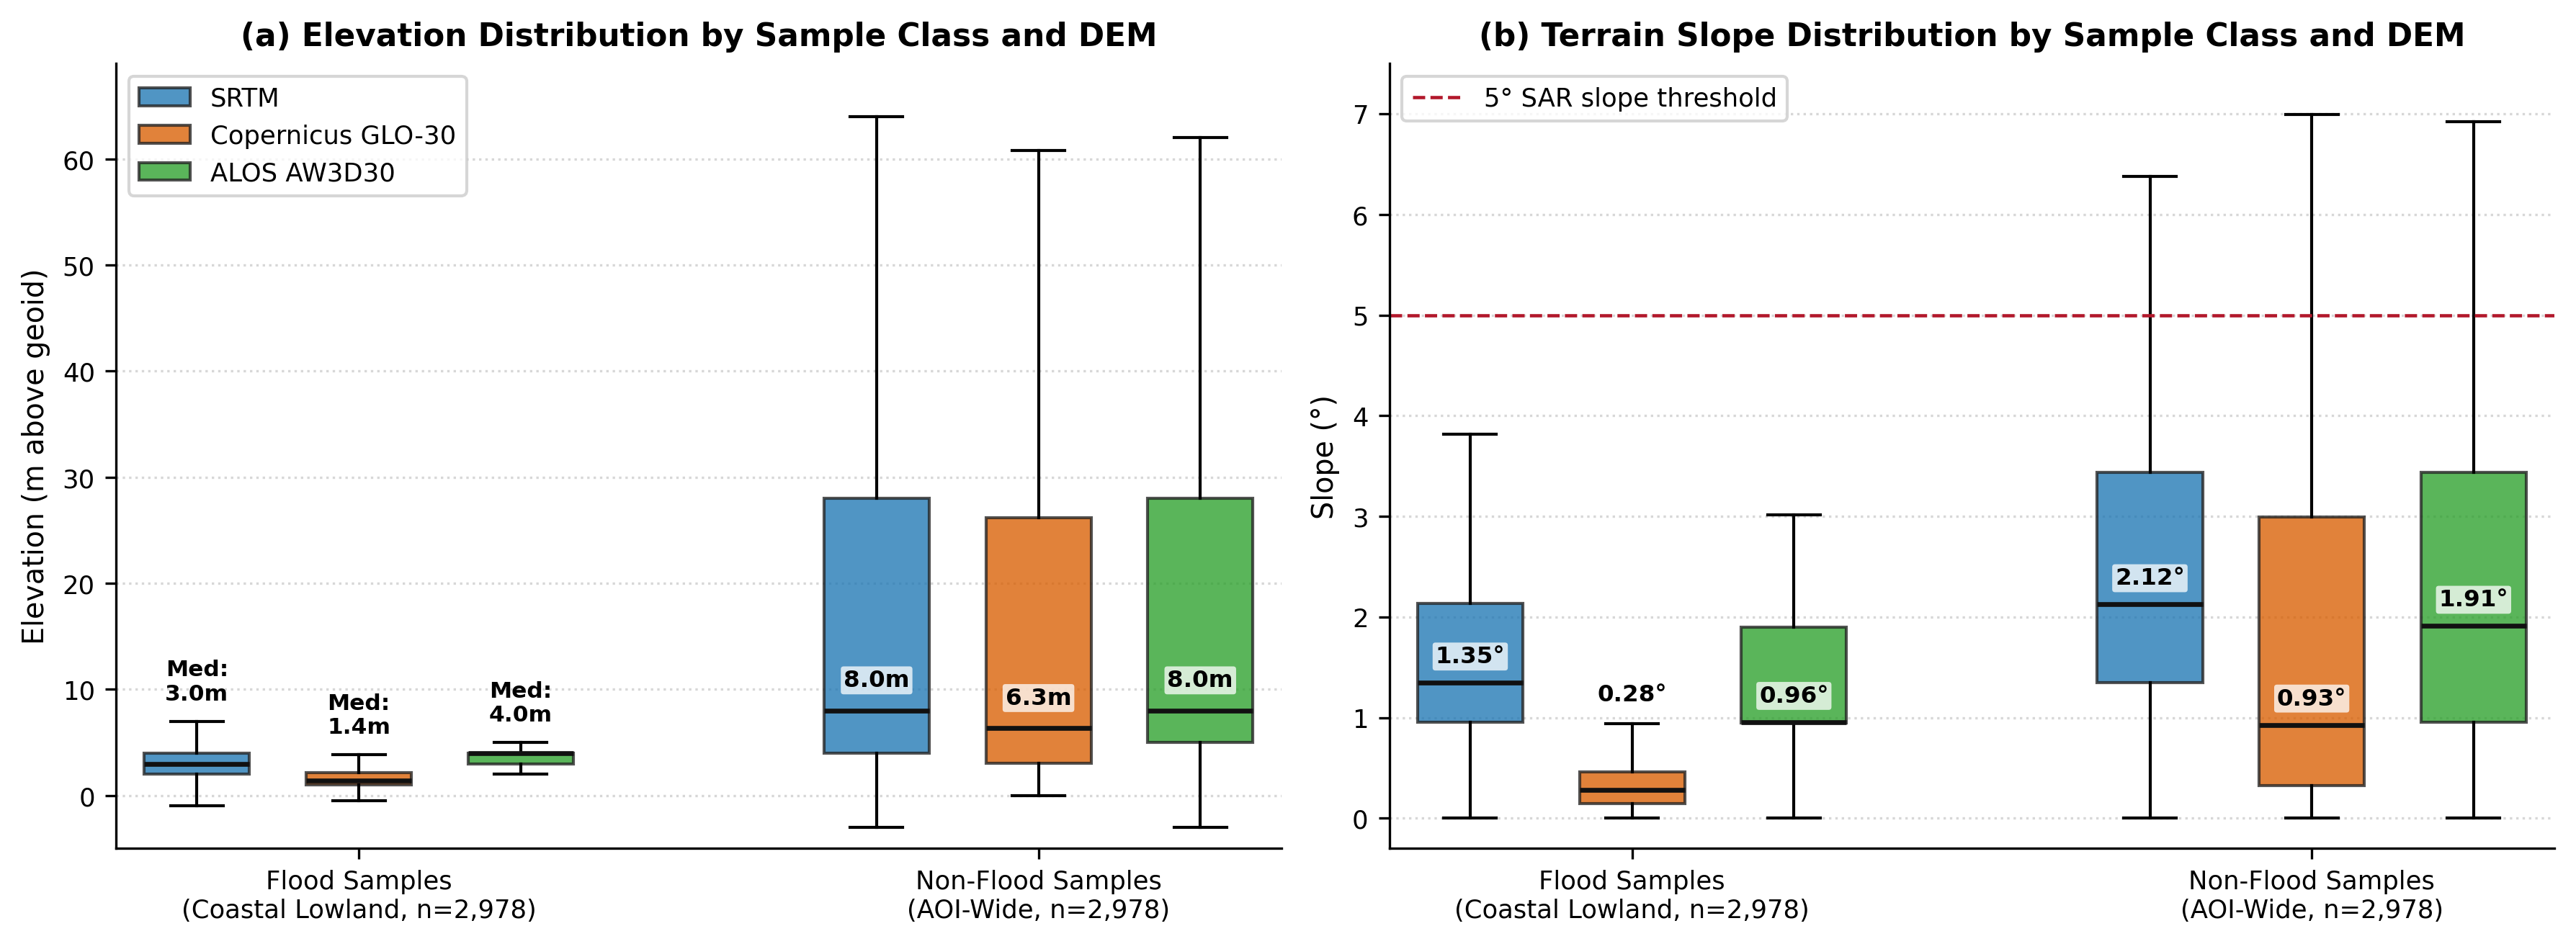
\includegraphics[width=0.94\textwidth]{figures/fig_dem_characteristics.png}
\caption{Empirical distributions of (a) elevation and (b) terrain slope across flood ($n = 2{,}978$) and non-flood ($n = 2{,}978$) master sample points for SRTM, Copernicus DEM GLO-30, and ALOS AW3D30. Boxplots display median, interquartile range, and $1.5\times\text{IQR}$ whiskers.}
\label{fig:dem-characteristics}
\end{figure}

\subsection{Predictive Performance Under Stratified Holdout and Spatial Cross-Validation}\label{subsec:model-performance}

Table~\ref{tab:holdout-metrics} presents the predictive performance of the controlled Random Forest models on the 25\% stratified random holdout set ($n_{\text{test}} = 1{,}489$; seed = 42). All three global DEM configurations achieve strong classification performance, with ROC-AUC ranging from $0.9318$ (SRTM) and $0.9360$ (ALOS AW3D30) to $0.9404$ (Copernicus GLO-30). At the standard $t = 0.50$ threshold, Copernicus GLO-30 attains the highest accuracy ($0.8899$), precision ($0.8580$), recall ($0.9341$), and F1-score ($0.8945$), followed consistently by ALOS AW3D30 ($\text{F1} = 0.8833$) and SRTM ($\text{F1} = 0.8791$). Evaluating predictions at the Youden-optimal threshold ($t^* \in [0.495, 0.521]$) yields nearly identical rankings and metrics, with $\Delta\text{ROC-AUC}$ relative to SRTM of $+0.0086$ for Copernicus GLO-30 and $+0.0042$ for ALOS AW3D30.

\begin{table}[!htbp]
\small
\centering
\caption{Controlled Random Forest performance on the 25\% stratified random holdout test set ($n_{\text{test}} = 1{,}489$; seed = 42) at the standard threshold ($t = 0.50$) and Youden-optimal threshold ($t^*$).}
\label{tab:holdout-metrics}
\begin{adjustbox}{max width=\textwidth}
\begin{tabular}{l c cccc c cccc c}
\toprule
& & \multicolumn{4}{c}{\textbf{Standard Threshold ($t = 0.50$)}} & & \multicolumn{4}{c}{\textbf{Youden-Optimal Threshold ($t^*$)}} & \\
\cmidrule(lr){3-6} \cmidrule(lr){8-11}
\textbf{DEM Configuration} & \textbf{ROC-AUC} & \textbf{Accuracy} & \textbf{Precision} & \textbf{Recall} & \textbf{F1-Score} & $\boldsymbol{t^*}$ & \textbf{Accuracy} & \textbf{Precision} & \textbf{Recall} & \textbf{F1-Score} & $\boldsymbol{\Delta}\textbf{AUC vs.\ SRTM}$ \\
\midrule
SRTM & 0.9318 & 0.8744 & 0.8468 & 0.9140 & 0.8791 & 0.5205 & 0.8791 & 0.8588 & 0.9073 & 0.8824 & $0.0000$ \\
Copernicus GLO-30 & \textbf{0.9404} & \textbf{0.8899} & \textbf{0.8580} & \textbf{0.9341} & \textbf{0.8945} & 0.4953 & \textbf{0.8912} & 0.8584 & \textbf{0.9368} & \textbf{0.8959} & $+0.0086$ \\
ALOS AW3D30 & 0.9360 & 0.8784 & 0.8488 & 0.9207 & 0.8833 & 0.5209 & 0.8805 & 0.8555 & 0.9153 & 0.8844 & $+0.0042$ \\
\bottomrule
\end{tabular}
\end{adjustbox}
\end{table}

The confusion matrices at $t = 0.50$ (Figure~\ref{fig:confusion-matrices}) show that all three configurations maintain high sensitivity to the flood class (recall of $91.4\%\text{--}93.4\%$, corresponding to $680\text{--}695$ true positives out of $744$ flood test samples), while specificity on the non-flood class ranges from $83.5\%$ ($622/745$ for SRTM) to $84.6\%$ ($630/745$ for Copernicus GLO-30). Thus, substituting SRTM with Copernicus GLO-30 reduces false negatives by $23.4\%$ (from $64$ to $49$) while simultaneously reducing false positives from $123$ to $115$.

\begin{figure}[!htbp]
\centering
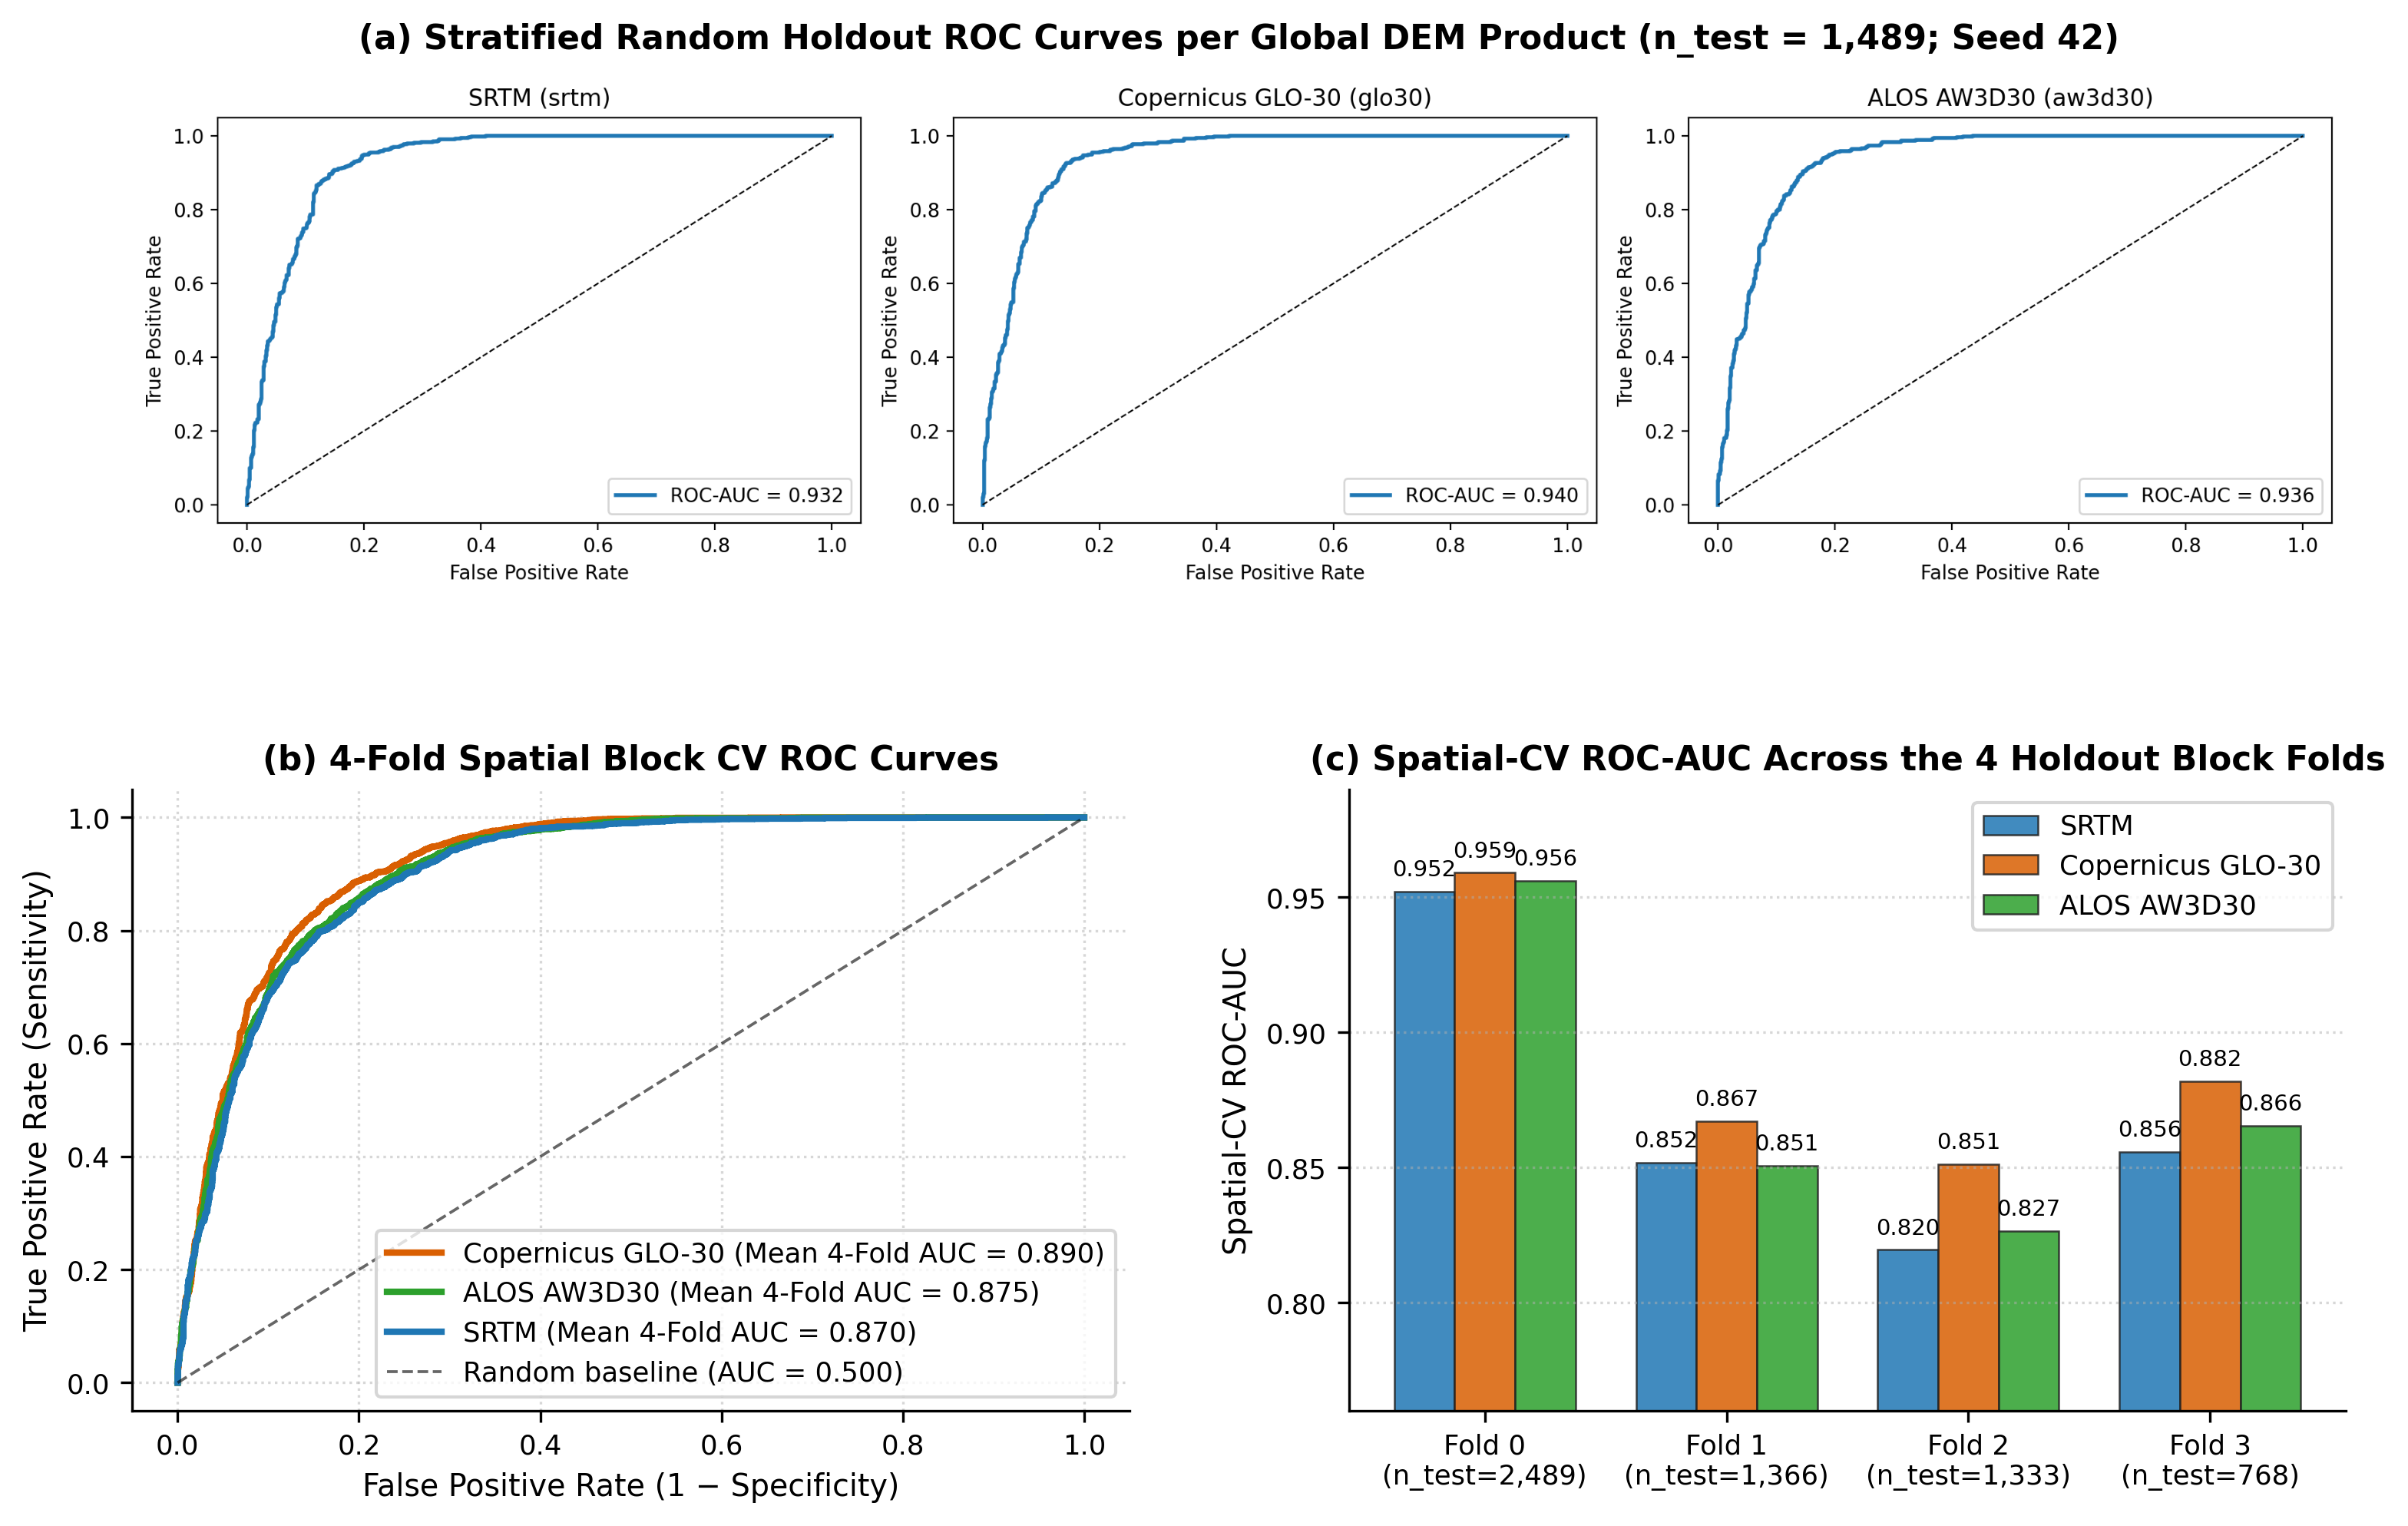
\includegraphics[width=0.94\textwidth]{figures/fig_roc.png}
\caption{ROC performance across evaluation protocols: (a) stratified random holdout ROC curves ($n_{\text{test}} = 1{,}489$; seed 42); (b) pooled four-fold spatial block cross-validation ROC curves; and (c) fold-by-fold spatial cross-validation ROC-AUC across the four held-out block groups.}
\label{fig:roc}
\end{figure}

\begin{figure}[!htbp]
\centering
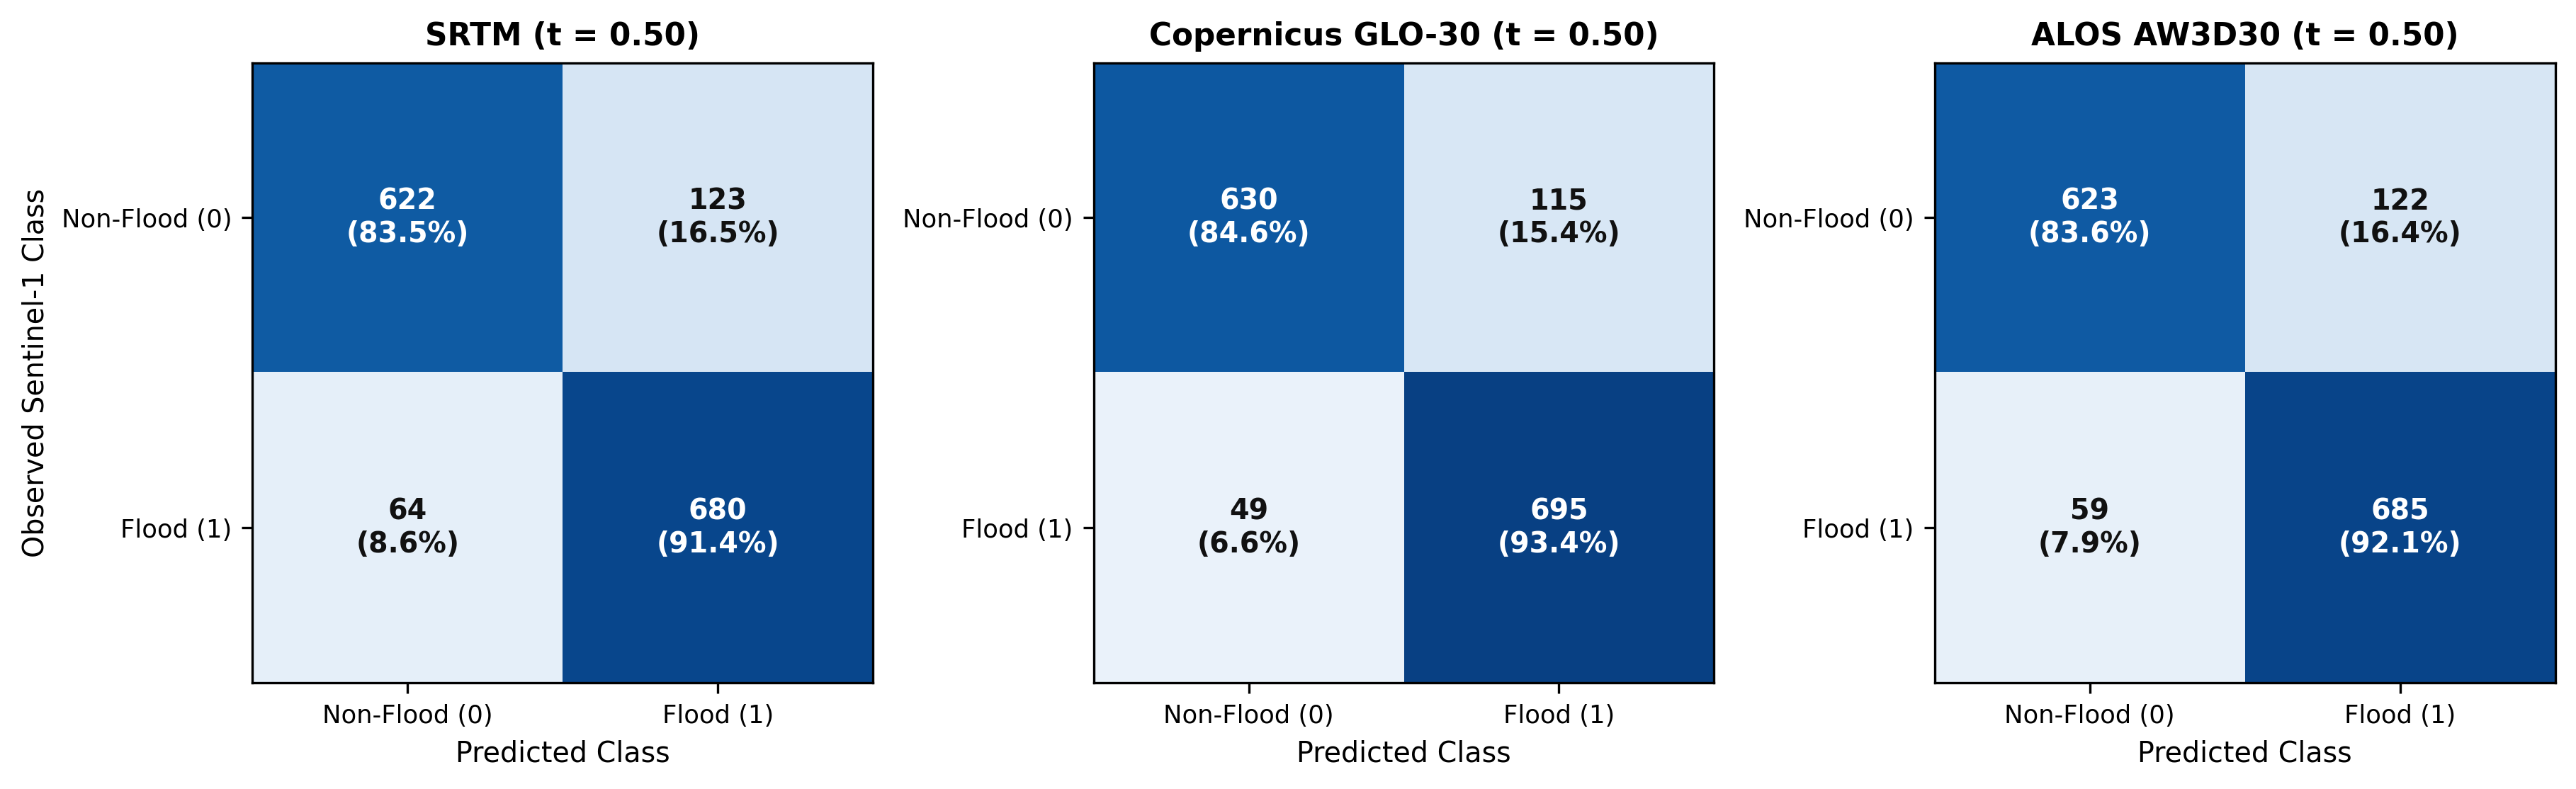
\includegraphics[width=0.94\textwidth]{figures/fig_confusion_matrices.png}
\caption{Held-out test set confusion matrices ($n_{\text{test}} = 1{,}489$; standard threshold $t = 0.50$) for SRTM, Copernicus DEM GLO-30, and ALOS AW3D30, reporting exact sample counts and row-normalized class percentages.}
\label{fig:confusion-matrices}
\end{figure}

When spatial autocorrelation between training and test points is suppressed via four-fold spatial block cross-validation across the 16 coordinate-quantile blocks (Table~\ref{tab:spatial-cv} and Figure~\ref{fig:roc}b--c), mean ROC-AUC decreases moderately by $\sim 0.05\text{--}0.06$ relative to random holdout, settling at $0.8699$ for SRTM, $0.8747$ for ALOS AW3D30, and $0.8899$ for Copernicus GLO-30. Notably, Copernicus GLO-30 achieves the highest probability-based ROC-AUC and F1-score in every individual spatial fold (Folds 0 through 3; Table~\ref{tab:spatial-cv}), demonstrating that its predictive advantage is preserved when extrapolating to spatially held-out blocks. Table~\ref{tab:spatial-cv} also illustrates the methodological importance of computing spatial CV ROC-AUC from continuous predicted probabilities ($\text{AUC}_{\text{prob}} = 0.870\text{--}0.890$) rather than binary hard predictions ($\text{AUC}_{\text{binary}} = 0.788\text{--}0.817$), as binary truncation underestimates ranking discrimination by $0.07\text{--}0.08$.

\begin{table}[!htbp]
\small
\centering
\caption{Four-fold spatial block cross-validation performance across the 16 coordinate-quantile blocks (seed = 42). $\text{AUC}_{\text{prob}}$ is computed from continuous predicted probabilities; $\text{AUC}_{\text{binary}}$ denotes legacy binary-threshold pseudo-AUC.}
\label{tab:spatial-cv}
\begin{adjustbox}{max width=\textwidth}
\begin{tabular}{c c c c l cccccc}
\toprule
\textbf{Fold} & \textbf{Held-Out Blocks} & $\boldsymbol{n_{\text{train}}}$ & $\boldsymbol{n_{\text{test}}}$ & \textbf{DEM Config} & $\textbf{AUC}_{\textbf{prob}}$ & $\textbf{AUC}_{\textbf{binary}}$ & \textbf{Accuracy} & \textbf{Precision} & \textbf{Recall} & \textbf{F1-Score} \\
\midrule
0 & $\{0, 1, 5, 14\}$ & 3,467 & 2,489 & SRTM & 0.9521 & 0.8667 & 0.8734 & 0.8755 & 0.8203 & 0.8470 \\
  & (Pos.\ rate: 42.7\%) & & & Copernicus GLO-30 & \textbf{0.9591} & \textbf{0.9047} & \textbf{0.9052} & 0.8797 & \textbf{0.9012} & \textbf{0.8903} \\
  & & & & ALOS AW3D30 & 0.9562 & 0.8870 & 0.8911 & \textbf{0.8830} & 0.8589 & 0.8708 \\
\midrule
1 & $\{8, 9, 11, 13\}$ & 4,590 & 1,366 & SRTM & 0.8519 & 0.7890 & 0.8302 & 0.8573 & \textbf{0.9014} & 0.8788 \\
  & (Pos.\ rate: 68.3\%) & & & Copernicus GLO-30 & \textbf{0.8673} & \textbf{0.8119} & \textbf{0.8360} & \textbf{0.8816} & 0.8778 & \textbf{0.8797} \\
  & & & & ALOS AW3D30 & 0.8508 & 0.7891 & 0.8184 & 0.8655 & 0.8692 & 0.8674 \\
\midrule
2 & $\{2, 4, 7, 15\}$ & 4,623 & 1,333 & SRTM & 0.8197 & 0.7279 & 0.7374 & \textbf{0.6939} & 0.6691 & 0.6812 \\
  & (Pos.\ rate: 41.9\%) & & & Copernicus GLO-30 & \textbf{0.8514} & \textbf{0.7523} & \textbf{0.7539} & 0.6928 & \textbf{0.7424} & \textbf{0.7168} \\
  & & & & ALOS AW3D30 & 0.8265 & 0.7177 & 0.7269 & 0.6796 & 0.6601 & 0.6697 \\
\midrule
3 & $\{3, 6, 10, 12\}$ & 5,188 & 768 & SRTM & 0.8559 & 0.7694 & 0.7669 & 0.8161 & 0.7447 & 0.7787 \\
  & (Pos.\ rate: 55.1\%) & & & Copernicus GLO-30 & \textbf{0.8820} & \textbf{0.7991} & \textbf{0.8008} & \textbf{0.8214} & \textbf{0.8156} & \textbf{0.8185} \\
  & & & & ALOS AW3D30 & 0.8655 & 0.7806 & 0.7812 & 0.8102 & 0.7872 & 0.7986 \\
\midrule
\multicolumn{4}{l}{\textbf{Mean Across 4 Spatial Folds}} & SRTM & 0.8699 & 0.7883 & 0.8020 & 0.8107 & 0.7839 & 0.7964 \\
\multicolumn{4}{l}{} & Copernicus GLO-30 & \textbf{0.8899} & \textbf{0.8170} & \textbf{0.8240} & \textbf{0.8189} & \textbf{0.8343} & \textbf{0.8263} \\
\multicolumn{4}{l}{} & ALOS AW3D30 & 0.8747 & 0.7936 & 0.8044 & 0.8096 & 0.7939 & 0.8016 \\
\bottomrule
\end{tabular}
\end{adjustbox}
\end{table}

\subsection{Statistical Significance via Block Bootstrap and Multi-Seed Robustness}\label{subsec:bootstrap-multiseed}

To evaluate whether the observed spatial cross-validation performance differences reflect genuine treatment effects rather than block-level sampling variability, Table~\ref{tab:bootstrap-multiseed} and Figure~\ref{fig:bootstrap-multiseed}a compare pairwise $\Delta\text{AUC}$ estimates under 16-block spatial bootstrap resampling against naive pixel-level bootstrap resampling. Under the primary 16-block spatial bootstrap, mean pooled ROC-AUC values are $0.8943$ (SRTM), $0.9098$ (Copernicus GLO-30), and $0.8990$ (ALOS AW3D30). Copernicus GLO-30 outperforms SRTM by $\Delta\text{AUC}_{\text{SRTM}-\text{GLO-30}} = -0.0155$ (95\% block CI $[-0.0250, -0.0072]$) and outperforms ALOS AW3D30 by $\Delta\text{AUC}_{\text{GLO-30}-\text{AW3D30}} = +0.0108$ (95\% block CI $[+0.0041, +0.0198]$). Because neither 95\% confidence interval crosses zero, the predictive advantage of Copernicus GLO-30 is statistically consistent across spatial blocks, albeit modest in magnitude ($\sim 0.011\text{--}0.016$ AUC). Conversely, the difference between SRTM and ALOS AW3D30 ($\Delta\text{AUC}_{\text{SRTM}-\text{AW3D30}} = -0.0047$, 95\% block CI $[-0.0096, +0.0013]$) includes zero under block resampling, indicating that SRTM and AW3D30 are statistically indistinguishable when accounting for spatial block dependence---even though naive pixel-level bootstrap ($\text{CI} = [-0.0074, -0.0023]$) would falsely declare the difference significant due to underestimated spatial variance.

\begin{table}[!htbp]
\small
\centering
\caption{Pairwise ROC-AUC differences ($\Delta\text{AUC}$) from 1,000-iteration paired 16-block spatial bootstrap versus pixel-level bootstrap, alongside multi-seed $\Delta\text{AUC}$ stability across five independent GEE runs ($\text{seeds} \in \{7, 42, 99, 100, 2024\}$).}
\label{tab:bootstrap-multiseed}
\begin{adjustbox}{max width=\textwidth}
\begin{tabular}{l rrrr rrr rr}
\toprule
& \multicolumn{4}{c}{\textbf{16-Block Spatial Bootstrap ($B=1{,}000$)}} & \multicolumn{3}{c}{\textbf{Pixel Bootstrap ($B=1{,}000$)}} & \multicolumn{2}{c}{\textbf{5-Seed Replication ($\text{Mean} \pm \text{SD}$)}} \\
\cmidrule(lr){2-5} \cmidrule(lr){6-8} \cmidrule(lr){9-10}
\textbf{DEM Pair Comparison} & $\boldsymbol{\Delta}\textbf{AUC}$ & \textbf{SD} & \textbf{95\% CI} & \textbf{Excludes 0?} & $\boldsymbol{\Delta}\textbf{AUC}$ & \textbf{95\% CI} & \textbf{Excludes 0?} & \textbf{Holdout $\boldsymbol{\Delta}$AUC} & \textbf{Spatial-CV $\boldsymbol{\Delta}$AUC} \\
\midrule
SRTM minus GLO-30 & $-0.0155$ & 0.0047 & $[-0.0250, -0.0072]$ & Yes & $-0.0141$ & $[-0.0173, -0.0109]$ & Yes & $-0.0082 \pm 0.0048$ & $-0.0200 \pm 0.0039$ \\
SRTM minus AW3D30 & $-0.0047$ & 0.0028 & $[-0.0096, +0.0013]$ & No (Marginal) & $-0.0048$ & $[-0.0074, -0.0023]$ & Yes (Overconfident) & $-0.0012 \pm 0.0021$ & $-0.0079 \pm 0.0034$ \\
GLO-30 minus AW3D30 & $+0.0108$ & 0.0042 & $[+0.0041, +0.0198]$ & Yes & $+0.0094$ & $[+0.0063, +0.0124]$ & Yes & $+0.0070 \pm 0.0027$ & $+0.0121 \pm 0.0055$ \\
\bottomrule
\end{tabular}
\end{adjustbox}
\end{table}

\begin{figure}[!htbp]
\centering
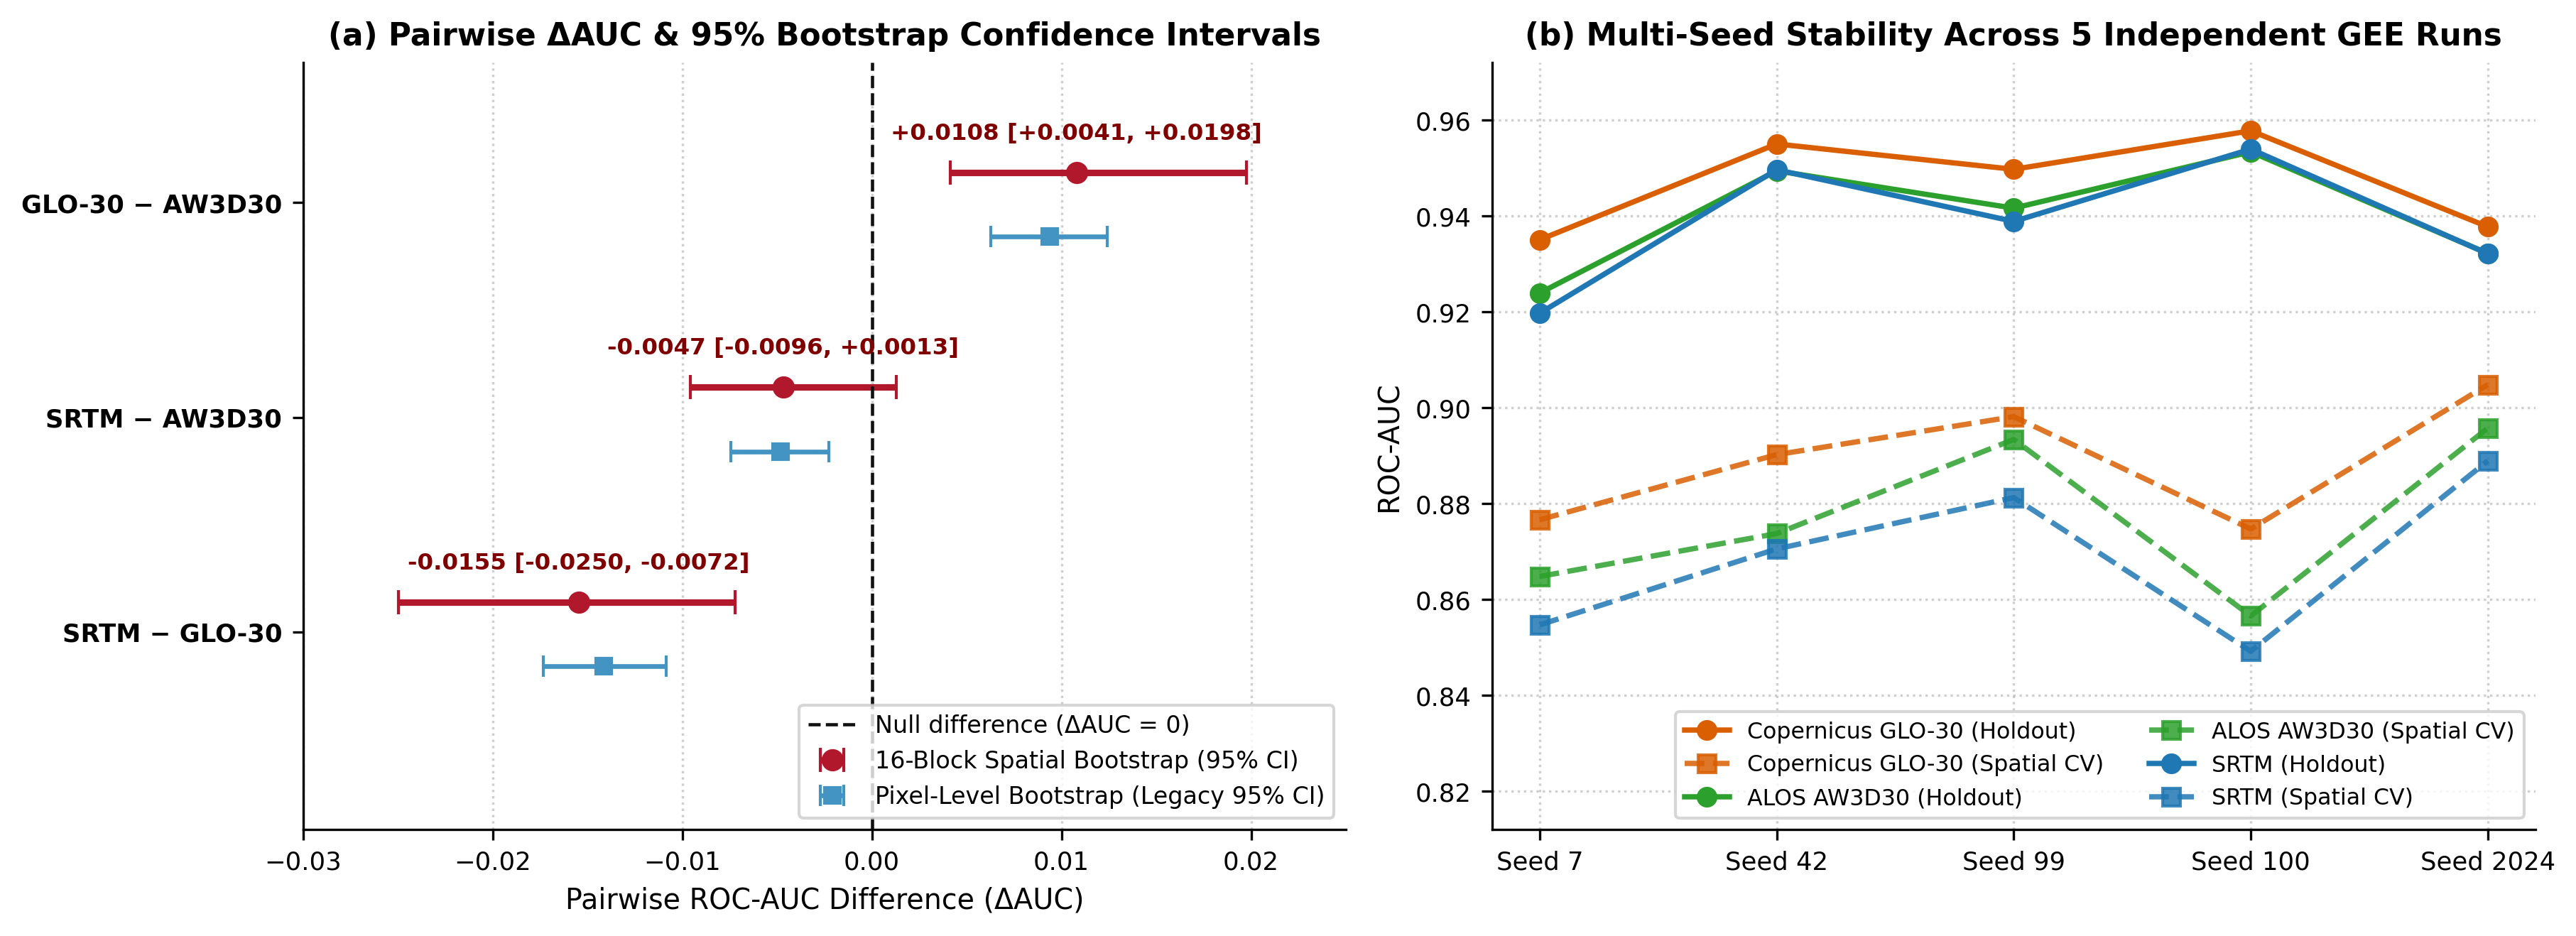
\includegraphics[width=0.94\textwidth]{figures/fig_bootstrap_multiseed.png}
\caption{Statistical inference and multi-seed stability: (a) pairwise $\Delta\text{AUC}$ point estimates and 95\% confidence intervals comparing 16-block spatial bootstrap against pixel-level bootstrap; (b) ROC-AUC trajectories across five independent end-to-end GEE sampling and modelling seeds ($7, 42, 99, 100, 2024$) for random holdout and four-fold spatial cross-validation.}
\label{fig:bootstrap-multiseed}
\end{figure}

End-to-end replication across five independent random seeds (Table~\ref{tab:multiseed-summary} and Figure~\ref{fig:bootstrap-multiseed}b) further confirms the stability of these findings. Across all five seeds, Copernicus DEM GLO-30 consistently ranks first in both random holdout ($\text{mean AUC} = 0.9471 \pm 0.0102$) and spatial block cross-validation ($\text{mean AUC} = 0.8889 \pm 0.0132$), outperforming ALOS AW3D30 ($0.9402 \pm 0.0121$ holdout; $0.8769 \pm 0.0173$ spatial CV) and SRTM ($0.9389 \pm 0.0138$ holdout; $0.8689 \pm 0.0169$ spatial CV). On spatial cross-validation, ALOS AW3D30 exceeds SRTM in every seed ($\Delta\text{AUC}_{\text{SRTM}-\text{AW3D30}} = -0.0079 \pm 0.0034$), whereas on random holdout SRTM is marginally higher than AW3D30 in two of the five seeds (seeds 42 and 100, by $\le 0.0006$; overall $\Delta\text{AUC} = -0.0012 \pm 0.0021$). Note also that the 1,000-iteration 16-block spatial bootstrap measures resampling variability across the 16 fixed spatial blocks rather than 1,000 independent spatial units.

\begin{table}[!htbp]
\small
\centering
\caption{Multi-seed robustness across five independent end-to-end GEE runs (seeds 7, 42, 99, 100, and 2024).}
\label{tab:multiseed-summary}
\begin{adjustbox}{max width=\textwidth}
\begin{tabular}{l ccccc c c}
\toprule
& \multicolumn{5}{c}{\textbf{Per-Seed Spatial-CV ROC-AUC (Holdout ROC-AUC in Parentheses)}} & \multicolumn{2}{c}{\textbf{5-Seed Summary ($\text{Mean} \pm \text{SD}$)}} \\
\cmidrule(lr){2-6} \cmidrule(lr){7-8}
\textbf{DEM Config} & \textbf{Seed 7} & \textbf{Seed 42} & \textbf{Seed 99} & \textbf{Seed 100} & \textbf{Seed 2024} & \textbf{Holdout AUC} & \textbf{Spatial-CV AUC} \\
\midrule
SRTM & 0.8547 (0.9197) & 0.8706 (0.9497) & 0.8813 (0.9389) & 0.8492 (0.9540) & 0.8890 (0.9322) & $0.9389 \pm 0.0138$ & $0.8689 \pm 0.0169$ \\
Copernicus GLO-30 & \textbf{0.8767} (\textbf{0.9351}) & \textbf{0.8902} (\textbf{0.9551}) & \textbf{0.8982} (\textbf{0.9498}) & \textbf{0.8747} (\textbf{0.9578}) & \textbf{0.9049} (\textbf{0.9378}) & $\mathbf{0.9471 \pm 0.0102}$ & $\mathbf{0.8889 \pm 0.0132}$ \\
ALOS AW3D30 & 0.8648 (0.9240) & 0.8738 (0.9495) & 0.8934 (0.9417) & 0.8566 (0.9534) & 0.8958 (0.9322) & $0.9402 \pm 0.0121$ & $0.8769 \pm 0.0173$ \\
\bottomrule
\end{tabular}
\end{adjustbox}
\end{table}

Two auxiliary diagnostic experiments provide crucial methodological context. First, when we restricted non-flood sampling to the un-unmasked JRC riparian belt ($8.76\%$ of the AOI), spatial cross-validation ROC-AUC dropped to $\sim 0.70$ across all three DEMs---a shift of $\Delta\text{AUC} \approx 0.17$ compared with the $\approx 0.01\text{--}0.02$ difference among DEM products. Second, when we re-extracted predictors at the exact $1{,}870$ sample coordinates and train--test split of the baseline SMDS study \cite{hakim2026} (where GEE archive reprocessing yielded 70\% label concordance), holdout ROC-AUC was $0.802$ for SRTM, $0.795$ for Copernicus GLO-30, and $0.792$ for ALOS AW3D30. Together, these diagnostics demonstrate that while Copernicus GLO-30 holds a consistent edge across AOI-wide samples, absolute model performance and fine-scale product rankings are substantially more sensitive to non-flood sampling domain definition than to the choice of 30\,m global DEM.

\subsection{Wall-to-Wall Spatial Sensitivity and Susceptibility Class Transitions}\label{subsec:spatial-sensitivity}

Pixel-by-pixel comparison across the AOI-masked Semarang--Demak rasters ($1{,}444{,}085$ valid pixels for SRTM and GLO-30; $1{,}429{,}582$ valid pixels for AW3D30; Table~\ref{tab:spatial-sensitivity} and Figures~\ref{fig:prob-maps}--\ref{fig:spatial-sensitivity}) reveals that small differences in global ROC-AUC translate into non-trivial spatial reclassifications. Overall five-class agreement is highest between SRTM and ALOS AW3D30 ($84.27\%$, with mean absolute probability difference $\overline{|\Delta p|} = 0.0371$), intermediate between Copernicus GLO-30 and ALOS AW3D30 ($81.52\%$, $\overline{|\Delta p|} = 0.0483$), and lowest between SRTM and Copernicus GLO-30 ($79.36\%$, $\overline{|\Delta p|} = 0.0556$). Thus, between $15.7\%$ and $20.6\%$ of all valid pixels across Semarang--Demak shift susceptibility class depending on which global DEM is selected.

\begin{figure}[!htbp]
\centering
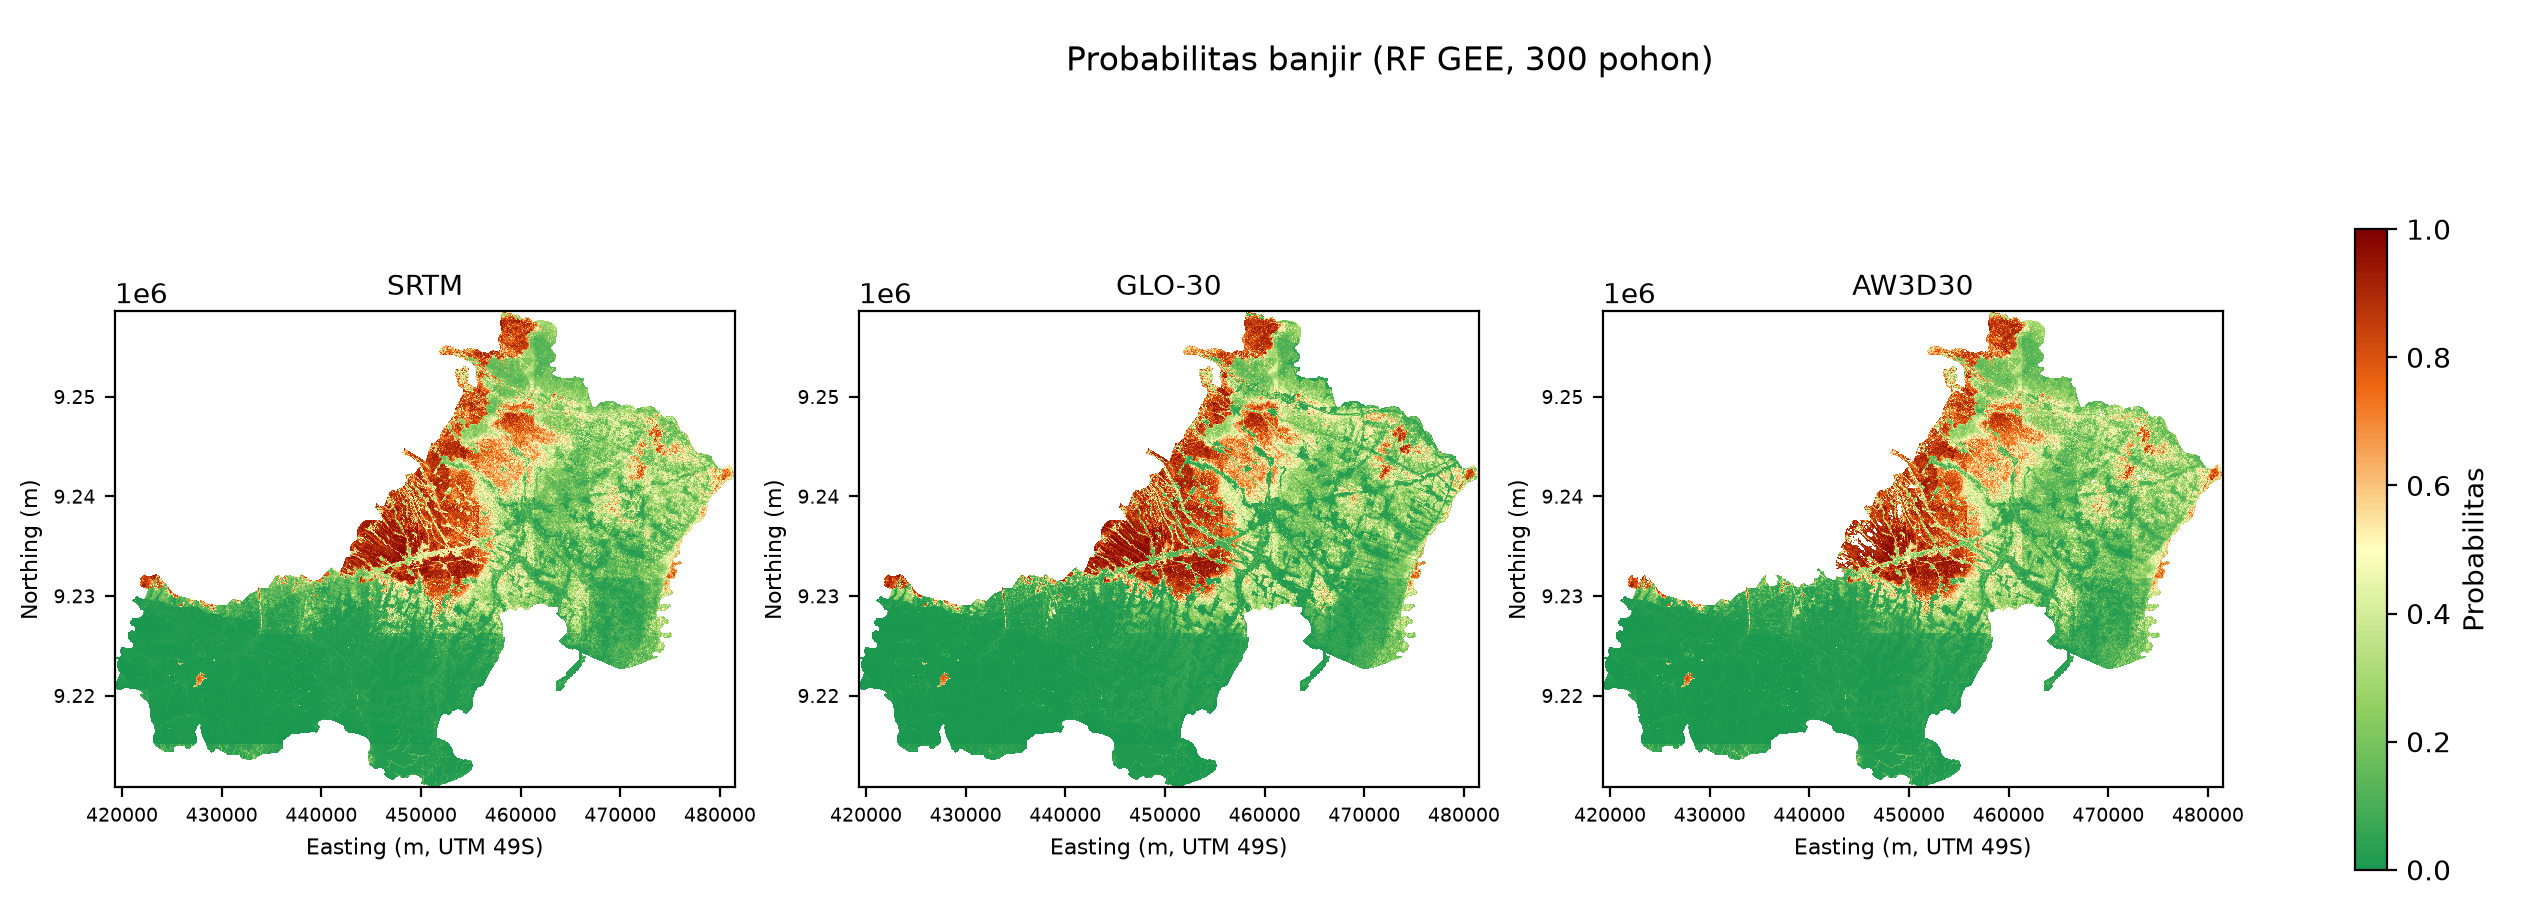
\includegraphics[width=0.96\textwidth]{figures/fig_prob_maps.png}
\caption{AOI-masked flood susceptibility probability maps ($p_d(x)$) across the Semarang--Demak coastal corridor derived from GEE \texttt{smileRandomForest} (300 trees) using SRTM, Copernicus DEM GLO-30, and ALOS AW3D30.}
\label{fig:prob-maps}
\end{figure}

\begin{table}[!htbp]
\small
\centering
\caption{Mapped area per flood susceptibility class ($\text{km}^2$ and \% of valid AOI) and pairwise spatial sensitivity summary across the AOI-masked Semarang--Demak domain.}
\label{tab:spatial-sensitivity}
\begin{adjustbox}{max width=\textwidth}
\begin{tabular}{l rrr rrr l cc}
\toprule
& \multicolumn{3}{c}{\textbf{Mapped Area ($\text{km}^2$)}} & \multicolumn{3}{c}{\textbf{Share of AOI (\%)}} & & \multicolumn{2}{c}{\textbf{Pairwise Spatial Sensitivity}} \\
\cmidrule(lr){2-4} \cmidrule(lr){5-7} \cmidrule(lr){9-10}
\textbf{Susceptibility Class (Probability Interval)} & \textbf{SRTM} & \textbf{GLO-30} & \textbf{AW3D30} & \textbf{SRTM} & \textbf{GLO-30} & \textbf{AW3D30} & \textbf{DEM Pair} & $\boldsymbol{\overline{|\Delta p|}}$ & \textbf{Class Agreement (\%)} \\
\midrule
Class 1: Very Low ($p \le 0.20$) & 756.71 & 822.64 & 772.46 & 58.22 & 63.29 & 60.03 & SRTM vs.\ GLO-30 & 0.0556 & 79.36\% \\
Class 2: Low ($0.20 < p \le 0.40$) & 233.13 & 189.85 & 222.06 & 17.94 & 14.61 & 17.26 & SRTM vs.\ AW3D30 & 0.0371 & 84.27\% \\
Class 3: Moderate ($0.40 < p \le 0.60$) & 114.08 & 98.47 & 108.18 & 8.78 & 7.58 & 8.41 & GLO-30 vs.\ AW3D30 & 0.0483 & 81.52\% \\
Class 4: High ($0.60 < p \le 0.80$) & 95.34 & 79.25 & 88.16 & 7.33 & 6.10 & 6.85 & & & \\
Class 5: Very High ($p > 0.80$) & 100.58 & 109.63 & 95.93 & 7.74 & 8.43 & 7.46 & & & \\
\midrule
\textbf{Total Valid AOI Area} & \textbf{1,299.84} & \textbf{1,299.84} & \textbf{1,286.79} & \textbf{100.00} & \textbf{100.00} & \textbf{100.00} & & & \\
\bottomrule
\end{tabular}
\end{adjustbox}
\end{table}

As shown in Table~\ref{tab:spatial-sensitivity} and Figure~\ref{fig:spatial-sensitivity}a, after strict AOI masking (which eliminates unmasked outside-AOI and nodata pixels from leaking into Class 5), Copernicus DEM GLO-30 produces a sharper bimodal polarization of susceptibility probabilities than SRTM, expanding both Class 1 (Very Low risk: $822.64\text{ km}^2$ vs.\ $756.71\text{ km}^2$ in SRTM, $+8.7\%$) and Class 5 (Very High risk: $109.63\text{ km}^2$ vs.\ $100.58\text{ km}^2$ in SRTM, $+9.0\%$) while contracting intermediate Classes 2--4. Conversely, ALOS AW3D30 contracts the Very High susceptibility zone to $95.93\text{ km}^2$ ($-4.6\%$ relative to SRTM), creating a net spread of $13.70\text{ km}^2$ ($14.3\%$) in priority flood hazard zoning depending solely on DEM selection. The transition matrices (Figure~\ref{fig:spatial-sensitivity}b--c) confirm that nearly all class shifts occur between adjacent susceptibility tiers: between SRTM and Copernicus GLO-30, the largest off-diagonal transitions are $94{,}306$ pixels shifting from Class 2 to Class 1 ($35.9\%$ of SRTM Class 2), $36{,}869$ pixels shifting from Class 1 to Class 2 ($4.3\%$), and $25{,}679$ pixels shifting upward from Class 4 to Class 5 ($23.9\%$ of SRTM Class 4), while extreme Class 1 $\leftrightarrow$ Class 5 jumps are virtually zero ($0\text{--}1$ pixel across the entire AOI).

\begin{figure}[!htbp]
\centering
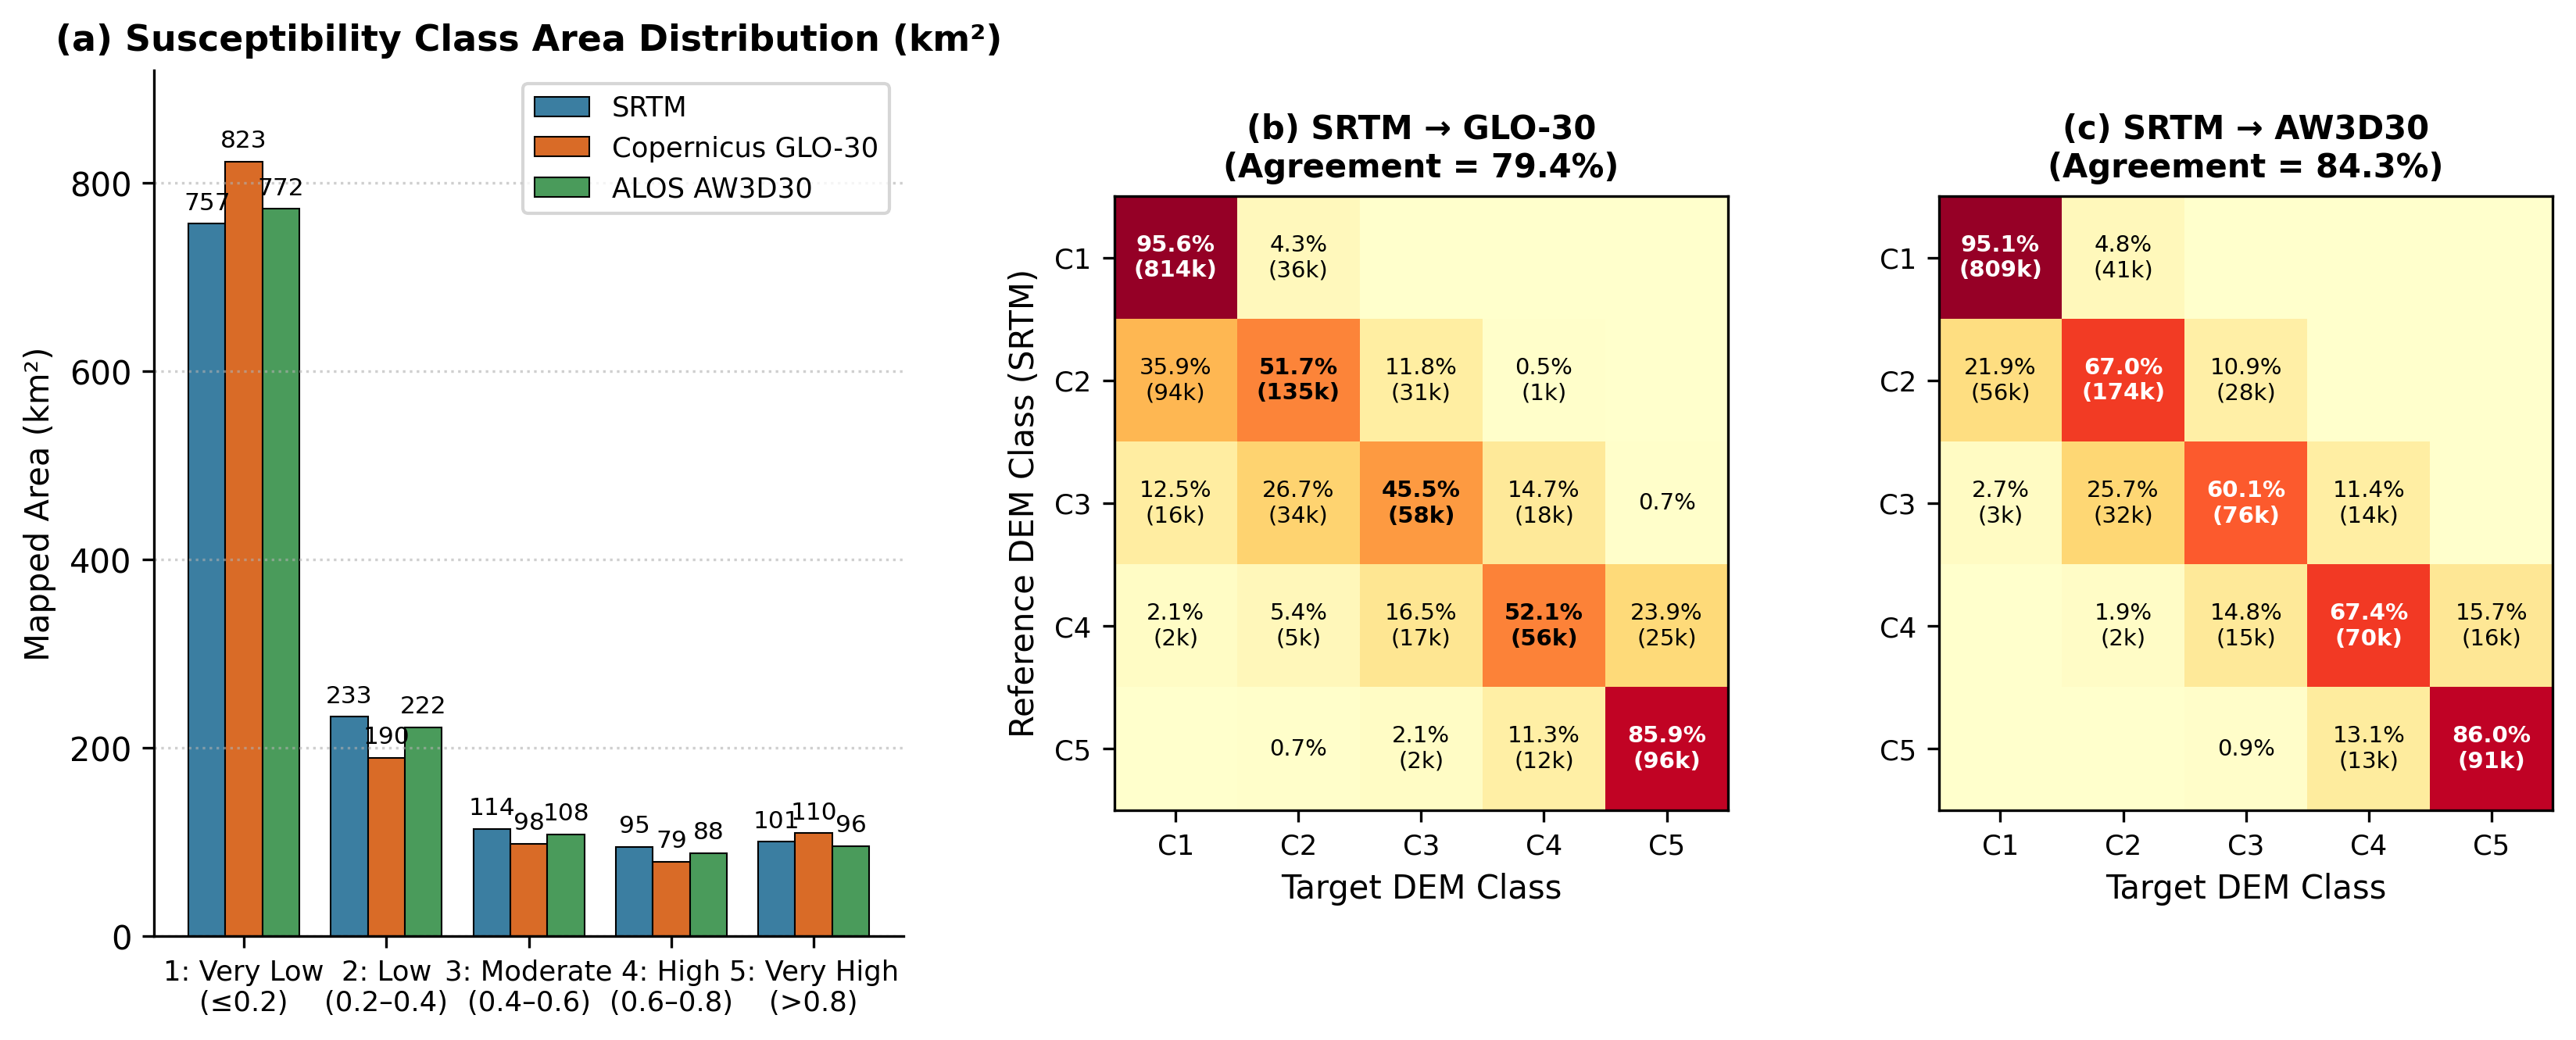
\includegraphics[width=0.94\textwidth]{figures/fig_spatial_sensitivity.png}
\caption{Wall-to-wall spatial sensitivity across the Semarang--Demak AOI: (a) mapped area ($\text{km}^2$) across the five equal-interval susceptibility classes; (b) pixel transition matrix from SRTM to Copernicus DEM GLO-30; and (c) pixel transition matrix from SRTM to ALOS AW3D30 (reporting row percentages and pixel counts in thousands).}
\label{fig:spatial-sensitivity}
\end{figure}

\subsection{Stratification of Spatial Sensitivity by ESA WorldCover Class}\label{subsec:worldcover-sensitivity}

Stratifying the pixel-wise sensitivity metrics across ESA WorldCover land-cover classes (Table~\ref{tab:worldcover-sensitivity} and Figure~\ref{fig:agreement}) demonstrates that DEM sensitivity is strongly conditioned by surface cover type. Across all three DEM pairs, \textbf{tree cover} (\texttt{lc\_10}) is the most stable land-cover stratum, achieving spatial class agreement of $95.61\%\text{--}96.87\%$ and the lowest mean absolute probability shift ($\overline{|\Delta p|} = 0.0113\text{--}0.0210$), primarily because forested areas in the AOI occupy steeper southern uplands where flood probability remains uniformly near zero regardless of minor DEM differences. \textbf{Built-up urban land} (\texttt{lc\_50}) is the second most stable stratum, with class agreement of $87.19\%\text{--}91.18\%$ and $\overline{|\Delta p|} = 0.0290\text{--}0.0514$.

\begin{table}[!htbp]
\small
\centering
\caption{Stratified spatial sensitivity across ESA WorldCover v200 land-cover classes for all three global DEM pairs.}
\label{tab:worldcover-sensitivity}
\begin{adjustbox}{max width=\textwidth}
\begin{tabular}{cl ccc ccc ccc}
\toprule
& & \multicolumn{3}{c}{\textbf{Mean Absolute Shift $\boldsymbol{\overline{|\Delta p|}}$}} & \multicolumn{3}{c}{\textbf{Class Agreement Rate (\%)}} & \multicolumn{3}{c}{\textbf{Class Changed Rate (\%)}} \\
\cmidrule(lr){3-5} \cmidrule(lr){6-8} \cmidrule(lr){9-11}
\textbf{Code} & \textbf{WorldCover Class} & \textbf{SRTM--GLO30} & \textbf{SRTM--AW3D30} & \textbf{GLO30--AW3D30} & \textbf{SRTM--GLO30} & \textbf{SRTM--AW3D30} & \textbf{GLO30--AW3D30} & \textbf{SRTM--GLO30} & \textbf{SRTM--AW3D30} & \textbf{GLO30--AW3D30} \\
\midrule
10 & Tree cover & 0.0210 & 0.0113 & 0.0170 & \textbf{95.61} & \textbf{96.78} & \textbf{96.87} & 4.39 & 3.22 & 3.13 \\
50 & Built-up & 0.0514 & 0.0290 & 0.0373 & 87.19 & 91.18 & 90.77 & 12.81 & 8.82 & 9.23 \\
30 & Grassland & 0.0538 & 0.0300 & 0.0484 & 78.25 & 86.65 & 80.86 & 21.75 & 13.35 & 19.14 \\
80 & Permanent water & 0.0600 & 0.0405 & 0.0582 & 76.87 & 84.09 & 77.95 & 23.13 & 15.91 & 22.05 \\
90 & Herbaceous wetland & 0.0609 & 0.0472 & 0.0574 & 72.46 & 78.29 & 74.24 & 27.54 & 21.71 & 25.76 \\
40 & Cropland & 0.0728 & 0.0526 & 0.0659 & 69.27 & 75.54 & 71.32 & 30.73 & 24.46 & 28.68 \\
60 & Bare / sparse veg.\ & 0.0877 & 0.0478 & 0.0717 & 63.07 & 78.13 & 68.59 & 36.93 & 21.87 & 31.41 \\
95 & Mangroves & 0.0749 & 0.0493 & 0.0774 & 62.79 & 74.87 & 62.64 & 37.21 & 25.13 & 37.36 \\
20 & Shrubland & \textbf{0.0943} & \textbf{0.0585} & \textbf{0.0915} & 59.07 & 75.41 & 57.57 & \textbf{40.93} & \textbf{24.59} & \textbf{42.43} \\
\bottomrule
\end{tabular}
\end{adjustbox}
\end{table}

In stark contrast, spatial sensitivity is highest in transitional coastal and agricultural vegetated surfaces: \textbf{shrubland} (\texttt{lc\_20}, where class agreement drops to $57.57\%$ between GLO-30 and AW3D30 and $59.07\%$ between SRTM and GLO-30, with $\overline{|\Delta p|}$ reaching $0.0943$), \textbf{mangroves} (\texttt{lc\_95}, $62.64\%\text{--}74.87\%$ agreement), \textbf{bare/sparse vegetation} (\texttt{lc\_60}, $63.07\%\text{--}78.13\%$ agreement), and \textbf{cropland} (\texttt{lc\_40}, $69.27\%\text{--}75.54\%$ agreement, meaning roughly $24.5\%\text{--}30.7\%$ of agricultural pixels change risk class across DEMs). Wetland (\texttt{lc\_90}) and water (\texttt{lc\_80}) occupy an intermediate regime ($72.46\%\text{--}84.09\%$ agreement).

\begin{figure}[!htbp]
\centering
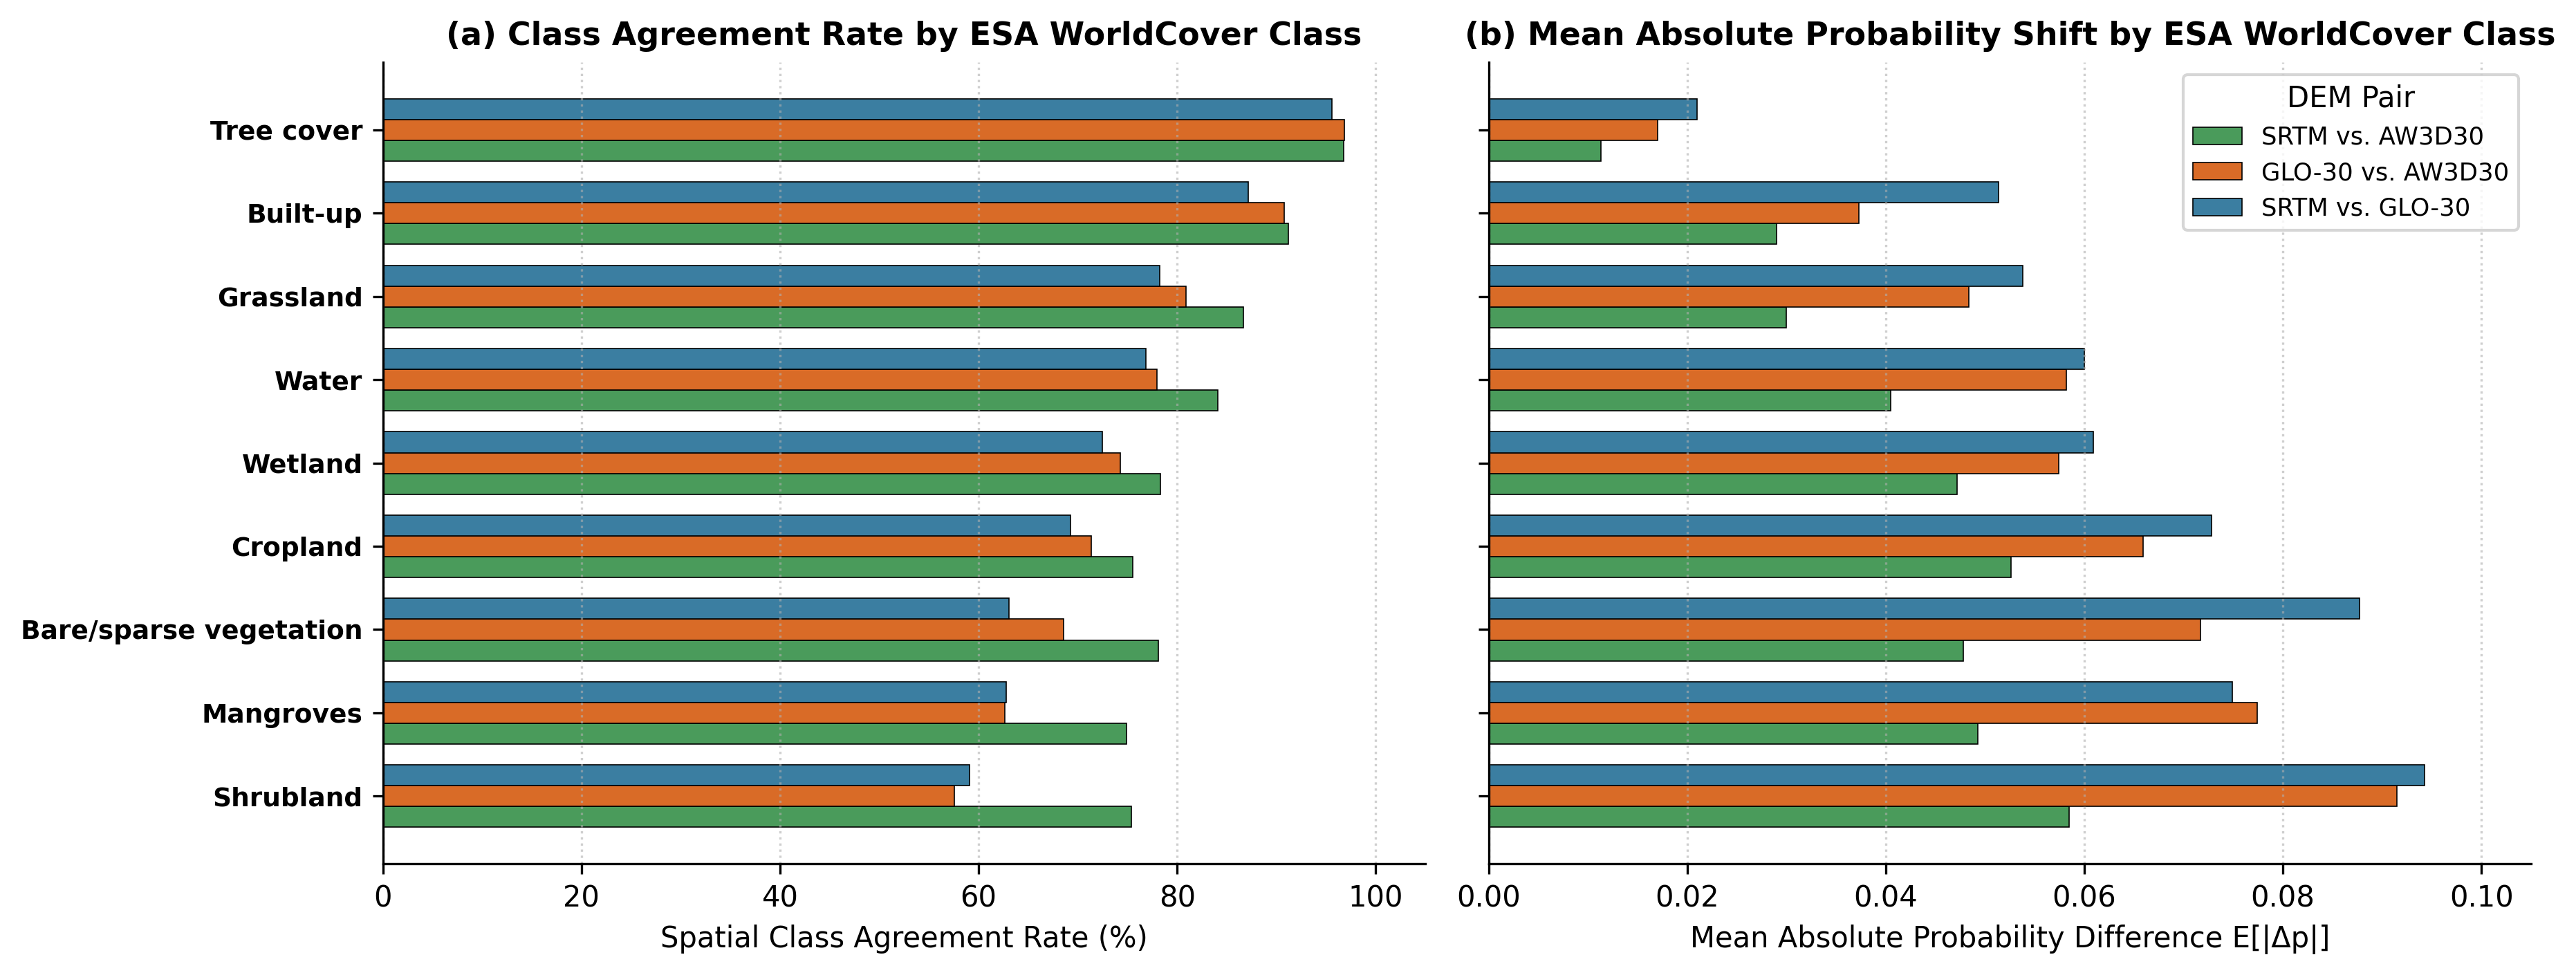
\includegraphics[width=0.94\textwidth]{figures/fig_agreement.png}
\caption{Stratified spatial sensitivity by ESA WorldCover land-cover class across the three DEM pairs: (a) five-class spatial agreement rate (\%); and (b) mean absolute probability difference $\overline{|\Delta p|}$.}
\label{fig:agreement}
\end{figure}

\subsection{Spatial Autocorrelation Diagnostics (Global Moran's $I$)}\label{subsec:moran-diagnostics}

Table~\ref{tab:moran-diagnostics} reports Global Moran's $I$ \cite{moran1950} across the sample points ($n = 5{,}956$; KNN $k=8$ in UTM 49S, $B = 9{,}999$ permutations, $E[I] = -0.000168$) and full AOI-masked probability rasters (Queen 8-neighbors, $B = 999$ permutations, \texttt{seed=42}). While the binary flood label ($I = 0.677$, $z = 109.7$) and out-of-fold predicted probabilities ($I = 0.877\text{--}0.886$) exhibit strong spatial clustering, the OOF residuals ($r_i = y_i - \hat{p}_i^{\text{OOF}}$) retain substantial positive spatial autocorrelation across all three models ($I = 0.377$ for SRTM, $0.355$ for GLO-30, and $0.364$ for AW3D30; all $p = 0.0001$), representing $52\%\text{--}56\%$ of the raw label clustering. Sensitivity checks across $k \in \{5, 8, 12\}$ confirm consistent residual clustering ($0.418, 0.377, 0.345$ for SRTM; $0.393, 0.355, 0.326$ for GLO-30; $0.405, 0.364, 0.334$ for AW3D30), with Copernicus GLO-30 consistently exhibiting the lowest residual autocorrelation. At the full raster level, all three GEE probability maps exhibit intense spatial clustering ($I = 0.9577$ for SRTM, $0.9531$ for GLO-30, and $0.9544$ for AW3D30; $p = 0.001$), explaining why random holdout validation overestimates generalization skill relative to spatial block cross-validation.

\begin{table}[!htbp]
\small
\centering
\caption{Global Moran's $I$ spatial autocorrelation diagnostics on sample OOF predictions/residuals ($n = 5{,}956$, KNN $k \in \{5,8,12\}$, $B = 9{,}999$) and AOI-masked GEE probability rasters (Queen 8-neighbors, $B = 999$).}
\label{tab:moran-diagnostics}
\begin{adjustbox}{max width=\textwidth}
\begin{tabular}{ll cccc ccc}
\toprule
& & \multicolumn{4}{c}{\textbf{Sample OOF Diagnostics ($n = 5{,}956$, $E[I]=-0.000168$)}} & \multicolumn{3}{c}{\textbf{AOI-Masked Probability Rasters (Queen 8)}} \\
\cmidrule(lr){3-6} \cmidrule(lr){7-9}
\textbf{DEM Configuration} & \textbf{Target} & \textbf{Moran's $\boldsymbol{I}$ ($k=8$)} & $\boldsymbol{z}$\textbf{-score} & \textbf{Resid.\ $\boldsymbol{I}$ ($k=5 / 8 / 12$)} & $\boldsymbol{p}$\textbf{-value} & \textbf{Valid Pixels ($n_{\text{used}}$)} & \textbf{Raster $\boldsymbol{I}$} & $\boldsymbol{z}$\textbf{-score ($p$)} \\
\midrule
Reference Label $y_i$ & Binary flood & 0.677 & 109.7 & --- & 0.0001 & --- & --- & --- \\
SRTM & $\hat{p}^{\text{OOF}}$ / $r^{\text{OOF}}$ & 0.886 / 0.377 & 143.6 / 61.4 & 0.418 / 0.377 / 0.345 & 0.0001 & 1,444,085 (0 isol.) & 0.9577 & 2,362.9 (0.001) \\
Copernicus GLO-30 & $\hat{p}^{\text{OOF}}$ / $r^{\text{OOF}}$ & 0.877 / \textbf{0.355} & 142.9 / \textbf{57.9} & \textbf{0.393} / \textbf{0.355} / \textbf{0.326} & 0.0001 & 1,444,085 (0 isol.) & 0.9531 & 2,351.7 (0.001) \\
ALOS AW3D30 & $\hat{p}^{\text{OOF}}$ / $r^{\text{OOF}}$ & 0.882 / 0.364 & 142.9 / 59.1 & 0.405 / 0.364 / 0.334 & 0.0001 & 1,429,580$^{\text{a}}$ (2 isol.) & 0.9544 & 2,252.0 (0.001) \\
\bottomrule
\multicolumn{9}{l}{\scriptsize $^{\text{a}}$Two isolated degree-0 pixels ($n_{\text{valid}} = 1{,}429{,}582$) excluded from row-standardized denominator $S_0 = n_{\text{used}}$.}
\end{tabular}
\end{adjustbox}
\end{table}

\FloatBarrier

%==================================
\section{Discussion}\label{sec:discussion}

\subsection{Topographic Representation and Predictive Sensitivity in Coastal Lowlands}\label{subsec:discussion-performance}

Our controlled experimental findings provide a clear answer to how global 30-meter elevation products influence machine learning flood susceptibility models in low-relief coastal environments. Addressing Research Question 1, SRTM, Copernicus DEM GLO-30, and ALOS AW3D30 exhibit consistent macro-topographic structure across Semarang--Demak, but diverge systematically within the low-lying northern plain where flooding occurs. Specifically, Copernicus DEM GLO-30 produces a lower median coastal elevation ($1.40\text{ m}$ at flood points vs.\ $3.00\text{ m}$ in SRTM and $4.00\text{ m}$ in AW3D30) and a markedly smoother slope distribution (median flood slope of $0.28^\circ$ vs.\ $1.35^\circ$ in SRTM and $0.96^\circ$ in AW3D30). This physical contrast reflects the underlying sensor physics: TanDEM-X single-pass bistatic X-band interferometry in Copernicus GLO-30 suppresses random phase speckle over flat alluvial plains, whereas C-band SRTM and optical stereo AW3D30 retain higher pixel-scale vertical noise that inflates local finite-difference slope calculations \cite{farr2007,tadono2016,esa_glo30,meadows2024}.

Addressing Research Questions 2 and 3, these topographic differences yield a small but statistically consistent hierarchy in predictive discrimination: Copernicus DEM GLO-30 $>$ ALOS AW3D30 $\ge$ SRTM. Because the flood inventory lives almost entirely on flat coastal terrain ($>98.7\%$ of flooded points have slopes $<5^\circ$), the reduced local slope noise and sharper lowland elevation gradient of Copernicus GLO-30 enable Random Forest trees to separate flood-prone coastal depressions from slightly higher non-flooded ground more cleanly. Crucially, our dual bootstrap analysis demonstrates why accounting for spatial autocorrelation is mandatory when comparing geospatial inputs \cite{roberts2017,ploton2020}: whereas naive pixel-level bootstrap resampling yields artificially narrow confidence intervals that declare all pairwise DEM differences significant, our 16-block spatial bootstrap confirms that Copernicus GLO-30's lead over SRTM ($\Delta\text{AUC} = +0.0155$) and AW3D30 ($\Delta\text{AUC} = +0.0108$) is robust to block resampling, while SRTM and AW3D30 are statistically indistinguishable ($\Delta\text{AUC} = -0.0047$, 95\% CI $[-0.0096, +0.0013]$).

\subsection{Spatial Divergence at Risk Class Boundaries and Land-Cover Dependence}\label{subsec:discussion-spatial}

A central practical takeaway of this study is that \textbf{small differences in global ROC-AUC ($\Delta\text{AUC} \approx 0.01\text{--}0.02$) do not imply spatial invariance of the resulting susceptibility maps}. Across the Semarang--Demak AOI, substituting SRTM with Copernicus GLO-30 alters the assigned five-level susceptibility class on $20.64\%$ of all valid AOI pixels ($\sim 268.3\text{ km}^2$) and shifts the area mapped as Very High susceptibility (Class 5) from $100.58\text{ km}^2$ in SRTM to $95.93\text{ km}^2$ in ALOS AW3D30 ($-4.6\%$) and $109.63\text{ km}^2$ in Copernicus GLO-30 ($+9.0\%$). For regional disaster-management agencies that prioritize mitigation budgets based on discrete high-risk zones \cite{fereshtehpour2024,Tique2026}, a $-4.6\%$ to $+9.0\%$ shift ($13.70\text{ km}^2$ spread) in the highest hazard tier represents a substantial change in prioritized land area.

Addressing Research Question 4, our WorldCover stratification explains where this spatial sensitivity originates. Rather than occurring uniformly, class disagreement is heavily concentrated in transitional coastal and agricultural land covers---shrubland (30.6\%--45.0\% class change), mangroves (27.0\%--38.0\%), bare/sparse coastal flats (24.5\%--36.4\%), and cropland (24.5\%--30.7%). In these low-gradient coastal zones, predicted flood probabilities frequently hover near the intermediate class thresholds ($0.20, 0.40, 0.60, 0.80$), and differential vegetation canopy penetration between C-band radar, X-band radar, and optical stereo photogrammetry introduces localized vertical biases \cite{meadows2024}. Conversely, upland tree cover ($>95.6\%$ agreement) and dense urban built-up cores ($87.2\%\text{--}91.2\%$ agreement) exhibit high inter-product stability because strong non-topographic signals (e.g., high elevation in uplands, impervious built-up spectral signatures, and permanent water proximity) anchor predictions firmly away from class boundaries.

\subsection{Methodological Insights, Limitations, and Future Directions}\label{subsec:discussion-limitations}

Beyond the primary DEM treatment comparison, our diagnostic experiments highlight a broader methodological lesson for remote-sensing susceptibility studies: \textbf{sampling domain definition can outweigh input sensor selection by an order of magnitude}. Correcting the sparse JRC permanent-water mask from a riparian-belt domain ($8.76\%$ of the AOI) to an AOI-wide domain ($97.95\%$ of non-flood pixels) increased spatial cross-validation ROC-AUC from $\sim 0.70$ to $0.870\text{--}0.890$ ($\Delta\text{AUC} \approx 0.17$), more than ten times the $\Delta\text{AUC}$ observed across the three global DEM products. Researchers using GEE water occurrence layers for non-flood masking must therefore explicitly unmask no-data pixels prior to boolean filtering to avoid severe domain-restriction bias.

Several limitations condition the interpretation of our results:
\begin{enumerate}
\item \textbf{Proxy SAR inventory and slope guard}: The supervisory target is derived from Sentinel-1 VH backscatter change detection for a single event (March 2024) rather than field-surveyed inundation boundaries, and employs an SRTM $<5^\circ$ slope guard. Although empirical auditing confirmed that $>98.7\%$ of flood samples lie below $5^\circ$ on all three DEMs (preventing material favouritism toward SRTM, which in fact ranked third), multi-event inventories with independent ground validation are needed to assess temporal generalizability.
\item \textbf{Shared hydrological baseline and uncorrected geoid datums}: Hydrological predictors (\texttt{hand}, \texttt{upa\_log}, \texttt{river\_width}, \texttt{dist\_river}) were locked from MERIT Hydro \cite{yamazaki2019} to maintain strict experimental control of non-treatment variables; deriving drainage networks independently from each raw DEM would test combined topographic--hydrological sensitivity \cite{Tique2026} but would confound direct DEM-feature attribution. Similarly, vertical datum offsets (EGM96 vs.\ EGM2008) were documented and retained in their native state; explicit geoid harmonization could be explored in future work.
\item \textbf{Granularity of spatial validation and dual RF engines}: Spatial block cross-validation relied on 16 coordinate-quantile blocks, and metric evaluation (\texttt{scikit-learn}, 400 trees) was paired with GEE raster classification (\texttt{smileRandomForest}, 300 trees). Finer spatial blocking schemes and dynamic coastal predictors (such as InSAR-derived land subsidence rates and tidal gauge stages \cite{abidin2015,yuwono2024}) should be integrated in future multi-temporal extensions.
\end{enumerate}

%==================================
\section{Conclusion}\label{sec:conclusion}

This study evaluated the sensitivity of Random Forest flood susceptibility mapping to three 30-meter global elevation products---SRTM, Copernicus DEM GLO-30, and ALOS AW3D30---in the Semarang--Demak coastal area under a strictly controlled experimental design. Four principal conclusions emerge:
\begin{enumerate}
\item \textbf{Topographic representation}: While all three DEMs capture the macro-scale coastal-to-upland gradient, they differ systematically in the low-lying flood domain, where Copernicus DEM GLO-30 exhibits lower median elevation ($1.40\text{ m}$ at flood points) and substantially lower local slope noise (median $0.28^\circ$) than ALOS AW3D30 ($4.00\text{ m}$, $0.96^\circ$) and SRTM ($3.00\text{ m}$, $1.35^\circ$).
\item \textbf{Controlled predictive performance}: All three DEM treatments yield strong flood discrimination on both stratified random holdout ($\text{ROC-AUC} = 0.932\text{--}0.940$) and four-fold spatial block cross-validation ($\text{ROC-AUC} = 0.870\text{--}0.890$), confirming that global 30-meter DEMs reliably support regional susceptibility screening when paired with multi-source GEE predictors.
\item \textbf{Statistical and spatial sensitivity}: Paired 16-block spatial bootstrap resampling and five-seed end-to-end replication confirm a modest but statistically consistent performance advantage for Copernicus DEM GLO-30 over both SRTM ($\Delta\text{AUC} = +0.0155$) and ALOS AW3D30 ($\Delta\text{AUC} = +0.0108$), whereas SRTM and ALOS AW3D30 are statistically indistinguishable under spatial block resampling. However, AOI-masked wall-to-wall raster comparisons show that 15.7\%--20.6\% of valid pixels change susceptibility class across DEM pairs, shifting the Very High risk class from $100.58\text{ km}^2$ (SRTM) to $95.93\text{ km}^2$ (AW3D30, $-4.6\%$) and $109.63\text{ km}^2$ (GLO-30, $+9.0\%$), while OOF residuals retain significant spatial autocorrelation (Moran's $I = 0.355\text{--}0.377$, $p = 0.0001$).
\item \textbf{Land-cover dependence}: Spatial sensitivity is highly heterogeneous across ESA WorldCover strata, remaining minimal in upland tree cover (95.6\%--96.9\% agreement) and urban built-up areas (87.2\%--91.2\%), but rising sharply in coastal shrubland (57.6\%--75.4\% agreement), mangroves (62.6\%--74.9\%), bare/sparse flats (63.1\%--78.1\%), and cropland (69.3\%--75.5\%). Practitioners mapping coastal flood susceptibility with open global DEMs should therefore prefer Copernicus DEM GLO-30 for lowland smoothness while explicitly accounting for class boundary uncertainty in vegetated coastal and agricultural zones.
\end{enumerate}

%==================================
\section*{Data Availability}
The complete Google Earth Engine and Python reproducible notebook (\texttt{Flood\_DEM\_Sensitivity\_Notebook\_v28.ipynb} and \texttt{T17\_Diagnostik\_Slope\_dan\_AOI\_v28.ipynb}), the balanced master sample dataset ($n = 5{,}956$ rows with all 27 extracted predictor bands), out-of-fold spatial cross-validation predictions, five-seed replication logs, block bootstrap tables, class transition matrices, and ESA WorldCover sensitivity tables are publicly archived and reproducible from the authors' repository and Google Earth Engine pipeline (\texttt{ee-irfan-banjir-2026}). All underlying satellite datasets (Sentinel-1 GRD, Sentinel-2 SR, SRTM GL1 v3, Copernicus DEM GLO-30, ALOS AW3D30 v4.1, MERIT Hydro, JRC Global Surface Water, CHIRPS Daily, and ESA WorldCover v200) are openly accessible via the Google Earth Engine public data catalog.

%==================================
\acknowledg{The authors thank the Department of Statistics and Data Science, Faculty of Mathematics and Natural Sciences, Universitas Negeri Semarang, for academic and computational support, and the European Space Agency (ESA), NASA/USGS, JAXA, and the Google Earth Engine team for providing open access to planetary-scale geospatial datasets.}

%==================================
\FloatBarrier
\printbibliography

\end{document}
